This chapter presents a sketch-based modeling system with auxiliary planes as references for 3D freeform shape design. The user first creates a rough 3D model of arbitrary topology by sketching some cross section curves of the model. Then the user can use sketching to perform deformation, extrusion, etc, to edit the model. To regularize and interpret the user's inputs properly, we introduce some rules for the strokes into the system, which are based on both the semantic meaning of the sketched strokes and human psychology. Unlike other sketching systems, all the creation and editing operations in the presented system are performed with reference to some auxiliary planes that are automatically constructed based on the user sketches or default settings. The use of reference planes provides a heuristic solution to the problem of ambiguity of 2D interface for modeling in 3D space. Examples demonstrate that the presented system can allow the user to intuitively and intelligently create and edit 3D models even with complex topology, which is usually difficult in other similar sketch-based modeling systems.



\section{Introduction}\label{ch3:sec:intro}

Creating and editing 3D models is a fundamental task in geometric modeling and computer graphics. Meanwhile it is also a tedious process with traditional 3D modeling packages such as Maya, 3DS Max and SolidWorks, which use the WIMP-style (Windows, Icon, Menu, Pointer) interfaces to construct and manipulate 3D models in a highly careful and skillful manner. The process and interactions in these packages are far from designers' habits and environments, since an intuitive modeling system should enable the user to communicate about any free-form shape in mind as quickly as with real-world
tools. 

In practice, designers often use sketches to design objects and present their ideas. Sketch-based modeling allows users to do modeling by simple sketches and gestures, which thus provides a new way for 3D modeling. It is suitable for early conceptual design and idea communication. A distinguished feature of sketch-based modeling over conventional modeling methods is the use of freeform curves (or strokes)as the basic modeling metaphor, which also propose some challenges. One of them is how to interpret and map the user sketched strokes, which is usually difficult. However, proper interpretation of sketching is very important because it is related to whether the system correctly understands the user's intention and whether the creation and editing is successfully performed. Another challenging problem is that when we are doing 3D modeling, we have to find \textit{indirect} ways to interact with 3D space using the input devices operating on the 2D computer screen. A classical solution to this problem is to use the Arcball~\cite{SK07} when we view a 3D object in a virtual environment rendered by some graphics library (such as OpenGL~\cite{SR06} or DirectX~\cite{BD06}). This problem becomes tougher for novice users who are not familiar or sensitive with 3D space when doing 3D modeling using sketches. It is very difficult, if not impossible, to specify the 3D position and orientation when sketching strokes into free space.

In this chapter, we propose methods to solve these problems. First, to partially eliminate the ambiguity of understanding the user input sketches, we introduce some rules for regularizing and interpreting them. These rules consider both the semantic meaning of the sketched strokes and human psychology. Second, to make the location and orientation of strokes in 3D space meaningful and intuitive, our guiding idea is to provide some reference geometry, with reference to which the strokes were sketched. In particular, we use the shape in its current design stage and also some auxiliary planes as reference geometry. The auxiliary planes are automatically constructed based on user's sketches or default settings. Figure~\ref{fig:screendeformpro} is an example where we want to deform the model by modifying the marked curve lying on it. It is not easy to give a precise description of the new position of the deformed 3D curve by sketching without any reference. With a reference plane constructed from the initial marked curve, the specification of the new curve becomes easier. Some assisting functions, such as the visual cue (previewed shape, hint points) display, automatic view rotation, intelligent stroke recognition and so on are designed to guide the user follow the rules and sketch in 3D space in an intuitive and flexible manner. Third, to improve the quality of the reconstructed mesh, we also introduce a local mesh refinement algorithm. It is mentioned in the survey~\cite{OSSJ09} that the model quality is one of five major open problems in sketch-based interface and modeling. Finally, by integrating all these techniques, we present a novel sketching interface for creating and editing 3D models. It is demonstrated that with help of reference planes, the sketch-based 3D modeling becomes more flexible and easier, thus leading to a more enjoyable touch of 3D space for users.

\begin{figure} [htbp]
  \centering
  \subfigure[]{
    \centering
    \label{fig:screendeformpro:a} %% label for first subfigure
    \begin{minipage}[b]{0.2\textwidth}
      \centering
      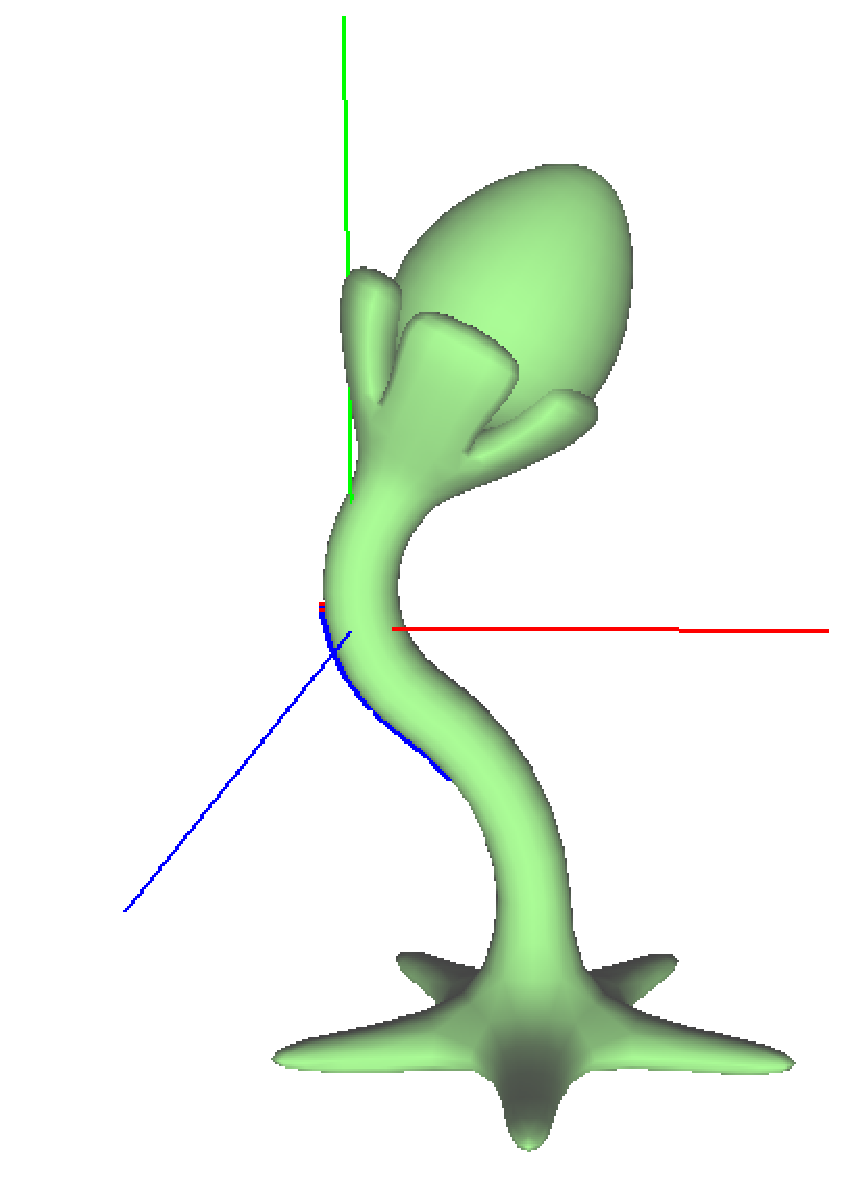
\includegraphics[scale=0.2]{figs/f3.2.a.eps}
    \end{minipage}}
  \subfigure[]{
    \centering
    \label{fig:screendeformpro:b}
    \begin{minipage}[b]{0.2\textwidth}
      \centering
      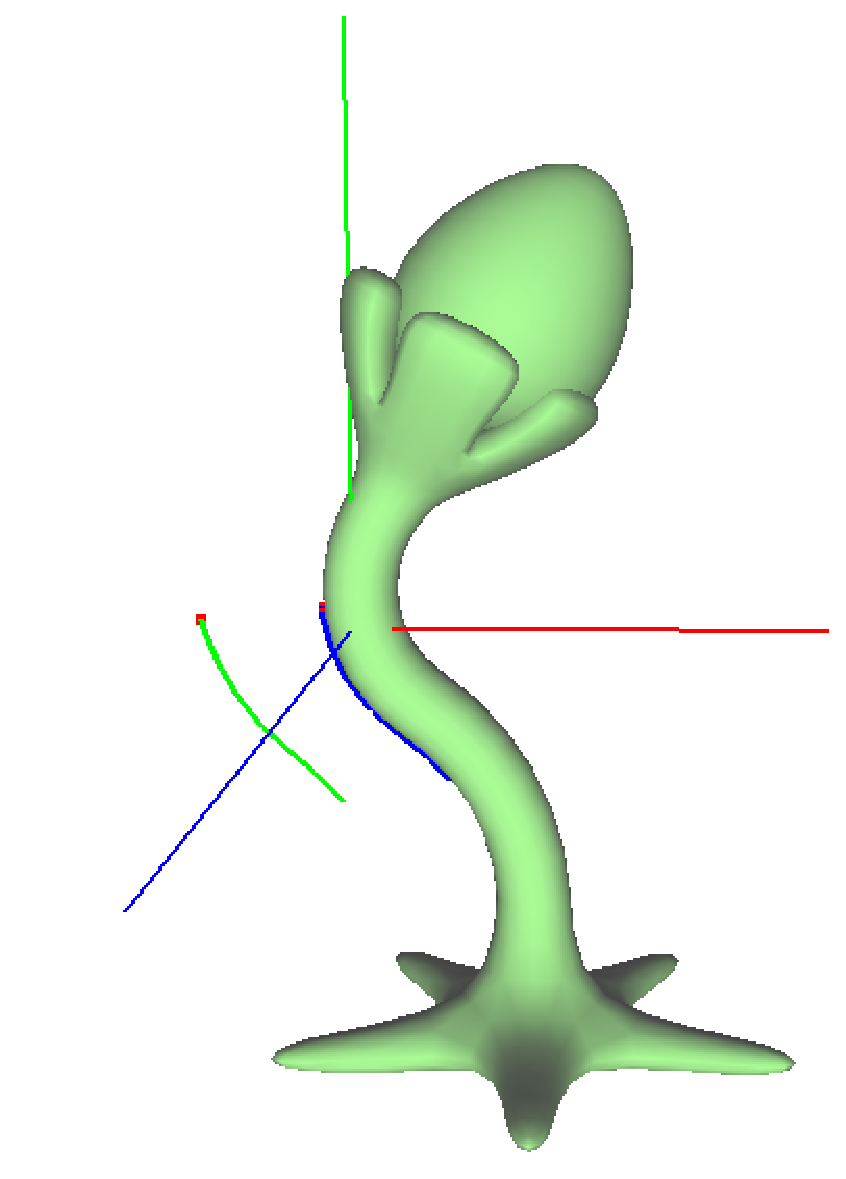
\includegraphics[scale=0.2]{figs/f3.2.b.eps}
    \end{minipage}}
  \subfigure[]{
    \centering
    \label{fig:screendeformpro:c}
    \begin{minipage}[b]{0.2\textwidth}
      \centering
      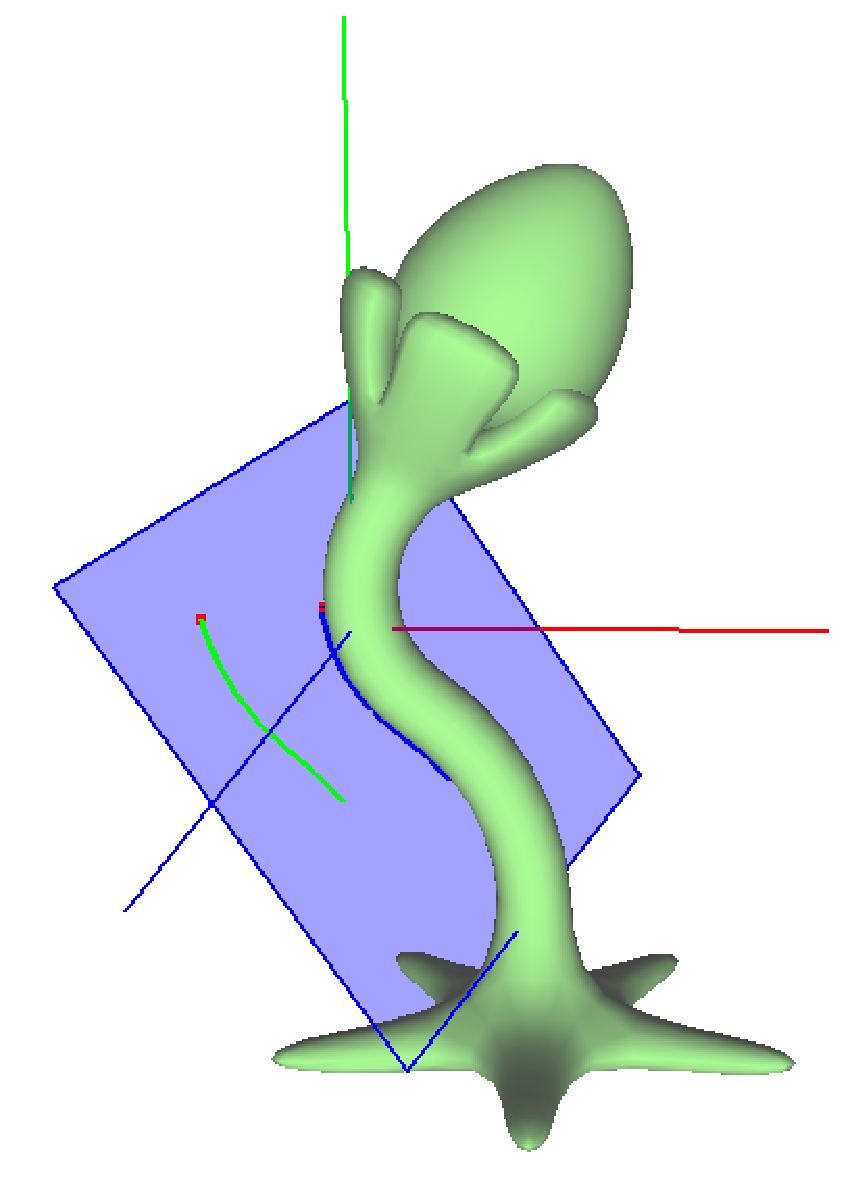
\includegraphics[scale=0.2]{figs/f3.2.c.eps}
    \end{minipage}}
  \subfigure[]{
    \centering
    \label{fig:screendeformpro:d}
    \begin{minipage}[b]{0.2\textwidth}
      \centering
      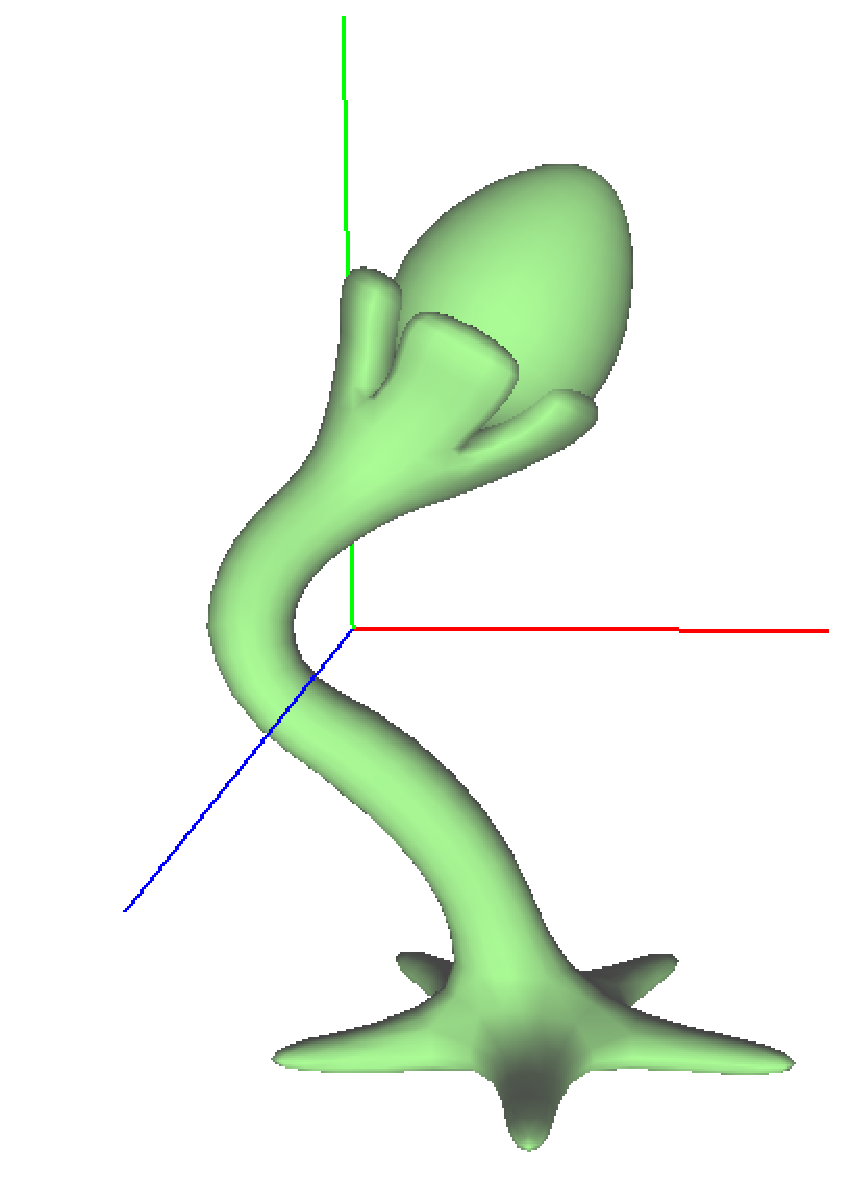
\includegraphics[scale=0.2]{figs/f3.2.d.eps}
    \end{minipage}}
  \caption{(a) In initial model and a handle stroke (blue curve) on it. (b) It is difficult to describe the position of the new handle stroke (in green color) in 3D space, which was sketched on the 2D screen. (c)Our system solved the problem by generating a reference plane (in blue color) for the user to sketch on. (d) Deformation result.}
  \label{fig:screendeformpro} %% label for entire figure
\end{figure}

The rest of this chapter is organized as follows: Chapter~\ref{ch3:sec:review} reviews some related works in sketch-based modeling and mesh deformation. Chapter~\ref{ch3:sec:ui} describes our sketching interface. The underlying algorithms that support and implement our sketching interface are explained in Chapter~\ref{ch3:sec:alg}. The experimental results are provided in Chapter~\ref{ch3:sec:result} and Chapter~\ref{ch3:sec:sum} concludes the chapter.

\section{Related Works}\label{ch3:sec:review}

Many sketch-based freeform modeling systems have been developed. One example is Teddy~\cite{IMT99}, which allows the user to draw a closed 2D contour and creates an initial model interpolating the contour. The generated model is a
simple oval-like object and a set of editing functions such as deformation, extrusion and cutting are provided to modify the rough shape to a satisfactory result. The final smooth surface is obtained through surface optimization. Similar works can be found in~\cite{KHR02,NISA07}. Touch-based techniques are also developed to sketch and modify contours of cross-sectional slices for modeling \lq\lq{blobby}\rq\rq 3D objects~\cite{JRPW10}.

The information of intersection of strokes sometimes helps to reconstruct 3D models. In order to model an object with some prescribed details from the 2D user sketches, CrossSketch~\cite{ASN07} first detects two intersected 2D strokes and then uses the Cubic Corners to reconstruct the depth of the vertices. It can generate a relatively complex 3D surface with more details while only able to construct an open surface rather than a closed 3D mesh. Masry and Lipson~\cite{ML07} present a system that is able to construct rigid 3D object consisting of both straight and cursive lines. The system first selects an intersection point of three edges as a central vertex and then reconstructs 3D straight lines using an optimization procedure, followed by the reconstruction of curves. This work provides an efficient way to model a rigid 3D object and is suitable for engineering design.

Some recent works propose to reconstruct 3D surfaces from closed curves lying on non-parallel planes~\cite{LBDLJ08,SLJGAGL09}. They are mainly applicable to regular predefined data such as the medical volume data of an organ of human body. However for the sketch-based free-form modeling application, the input strokes may not be regular and analyzing and processing of them may become quite complicated.

Besides the reconstruction of 3D models from initial input strokes, subsequent editings are usually desired to further modify the constructed models. We refer readers to an excellent survey paper~\cite{OSSJ09} for a broader overview. In the following we briefly look at some works on deformation.

To deform a constructed mesh, some sketch-based methods~\cite{NISA07,SCLARS04,SA07} let the user drag a vertex of the mesh along the direction parallel to the screen and then compute its position according to the position of the camera. The new positions of other vertices are computed using mesh deformation algorithms. This approach can give real-time feedback to the user and is suitable for interactive editing, but it is not intuitive enough for confirming the direction of deformation in 3D space. Meanwhile, it does not fit in the case where multiple handle vertices are desired.

Nealen et al~\cite{NSAC05} propose to deform a mesh by changing the shape of a handle curve. First a curve is drawn on the mesh to serve as the handle curve. Then the model is rotated manually to a proper angle and the deformed curve is drawn on the screen. The 3D position of the new curve could be calculated according to the current viewpoint. SilSketch~\cite{ZNA07} extends this idea by automatically detecting the handle curve which is a part of the silhouette of the model and corresponds to a user input stroke for the deformed handle curve. Similar method can also be found in~\cite{KSV09}.


\section{User Interface}\label{ch3:sec:ui}

Our sketching interface provides both the sketching and sculpting tools, which are the two techniques used in interactive shape modeling as introduced in~\cite{CIW08}, for the user to create and edit a 3D model. The sketching tool is used for creating the general shape of the model. The sculpting tool, which includes the deformation, extrusion, tunneling, cutting and smoothing functions can be used to make further editing. The selection of the function are done through intelligent stroke recognition. 

%-----------------------------------------------------------------------------------------------------------------
\subsection{Sketching Tool}\label{ch3:sec:ui:creation}

%FiberMesh: global re-computation after each edition, our system: can avoid this by using the subspace-based progressive modeling, each time a curve is sketched, the re-computation of the surface is only limited in the affected subspace, which makes our system well suited for quickly draft and improve a complex contour.
%For some modifications, for example, if the user sketches the detailed profile of a character and simply wants to bend the head a bit more, the only solution he has is to erase and re-draw the head from scratch. This is not easy to implement through only the sketching operation. So we also provide the sculpting tools for such editing operations.
%the preview function and calculated cross sections also help the user, especially artists to avoid imagination of the cross sections of an object, which is not intuitive for them and requires less engineering-type thinking.

Since most of previous free-form sketch-based modeling tools let the user to draw a 2D silhouette of a 3D object on the screen and then construct the 3D model by inflation and optimization~\cite{IMT99,KHR02,NISA07}, the initially generated shape is usually far from the desired one in the user's mind. In the general case of a complex, unknown free-form shape, the user usually needs to depict it from multiple viewpoints. Conventional 3D modeling softwares tackle this issue by providing orthogonal viewpoint windows, however, making sketching with several views seems much more technical and time consuming, especially for novice user who may easily get confused on 3D position and orientation. 

To solve this problem, we design a novel user interface, which provides the user three sets of orthogonal planes as the reference planes in the model creation stage. These reference planes are sketch planes, on which the user can sketch the cross sections of the model. The word \emph{cross section} means the intersection curve of the model with a plane. Initially, the $x=0$, $y=0$ and $z=0$ planes serve as the three basic orthogonal planes. The user can define the cross sections of a 3D model by sketching strokes on any of these basic planes.

\begin{figure} [htbp]
  \centering
  \subfigure[]{
    \centering
    \label{fig:uicreationEG:a} %% label for first subfigure
    \begin{minipage}[b]{0.23\textwidth}
      \centering
      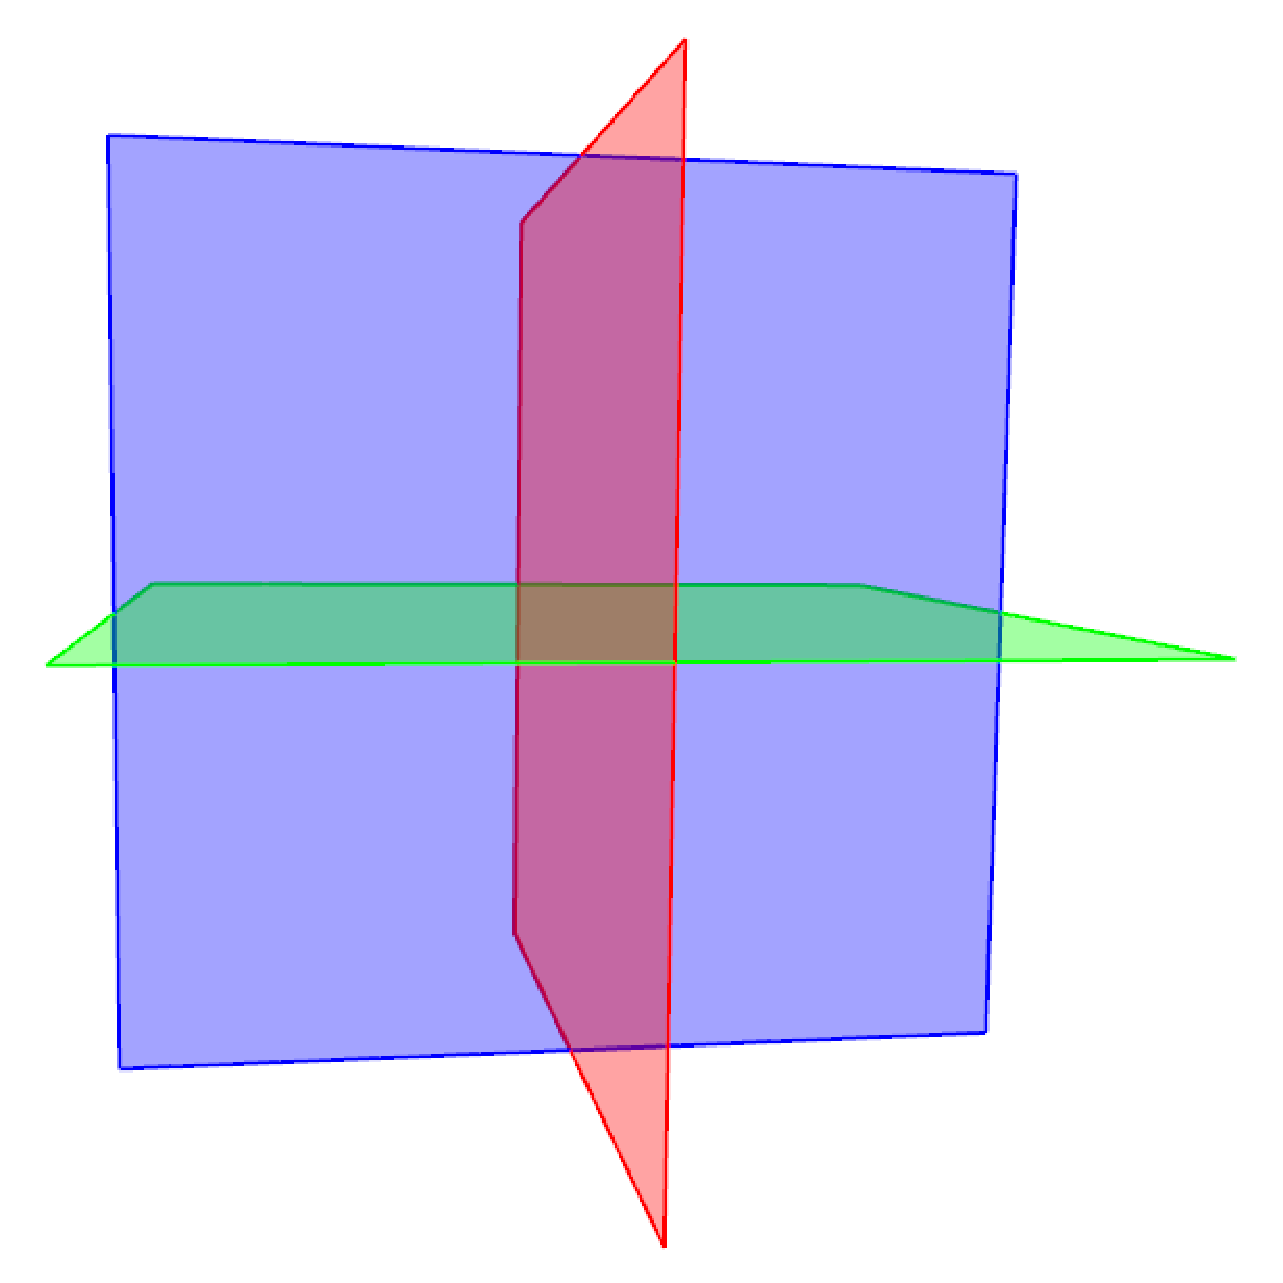
\includegraphics[scale=0.16]{figs/f3.3.3Hole1-ps.eps}
    \end{minipage}}
  \subfigure[]{
    \centering
    \label{fig:uicreationEG:b}
    \begin{minipage}[b]{0.23\textwidth}
      \centering
      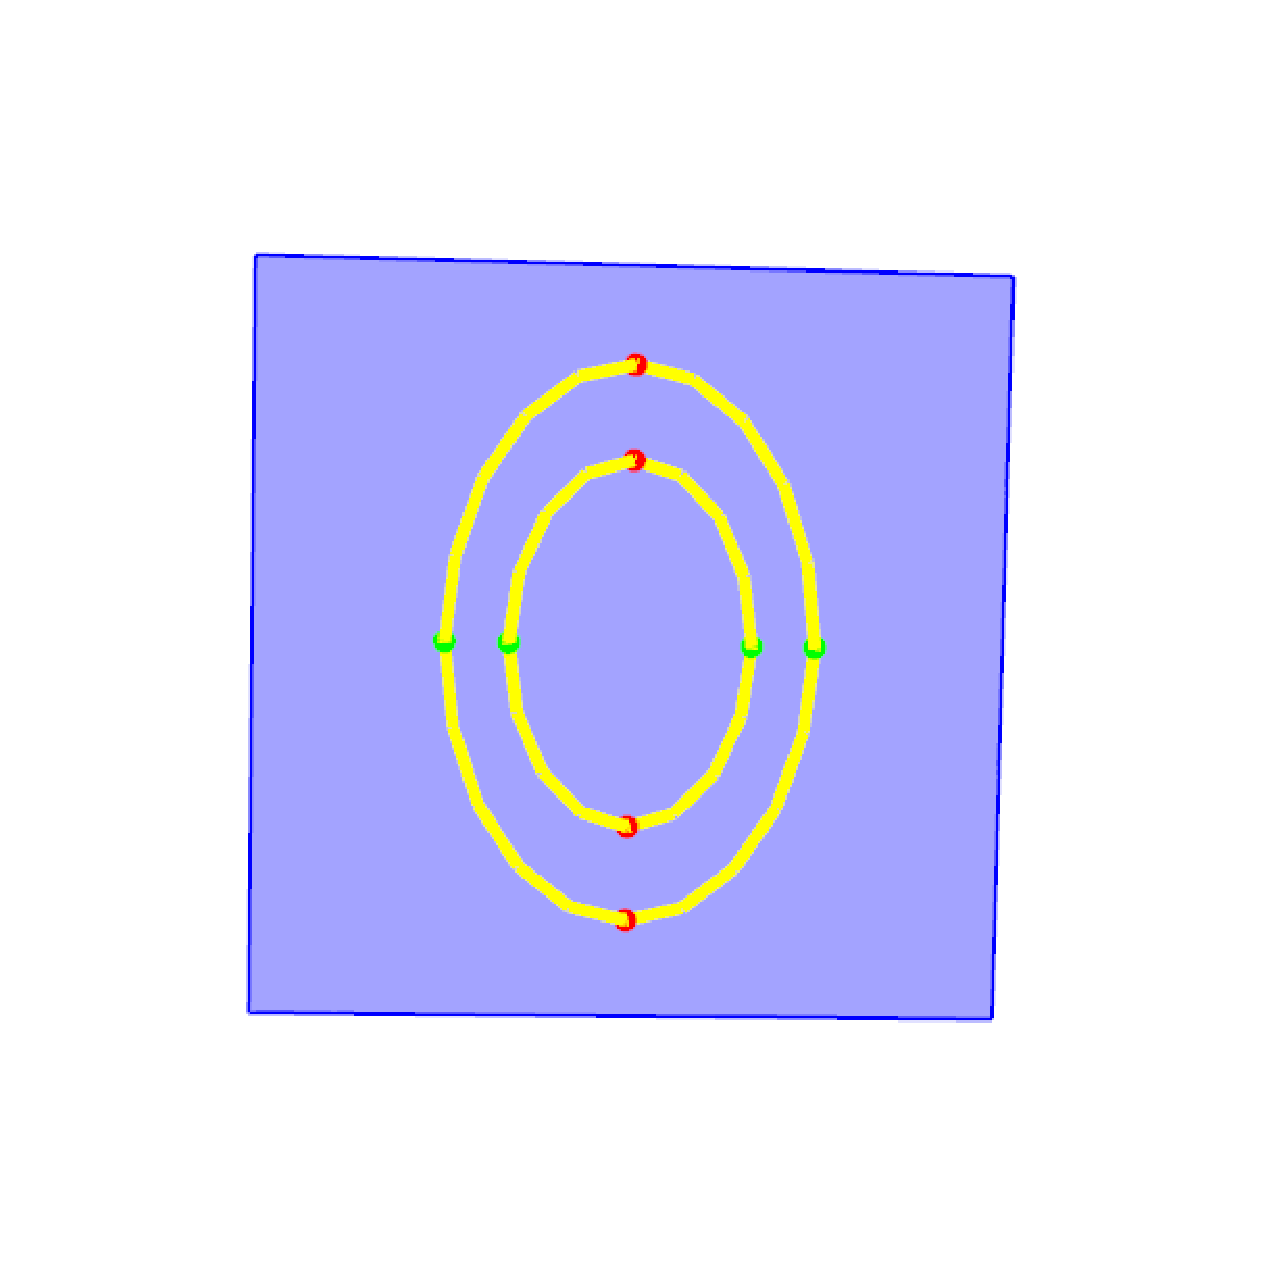
\includegraphics[scale=0.18]{figs/f3.3.3Hole2-ps.eps}
    \end{minipage}}
  \subfigure[]{
    \centering
    \label{fig:uicreationEG:c}
    \begin{minipage}[b]{0.23\textwidth}
      \centering
      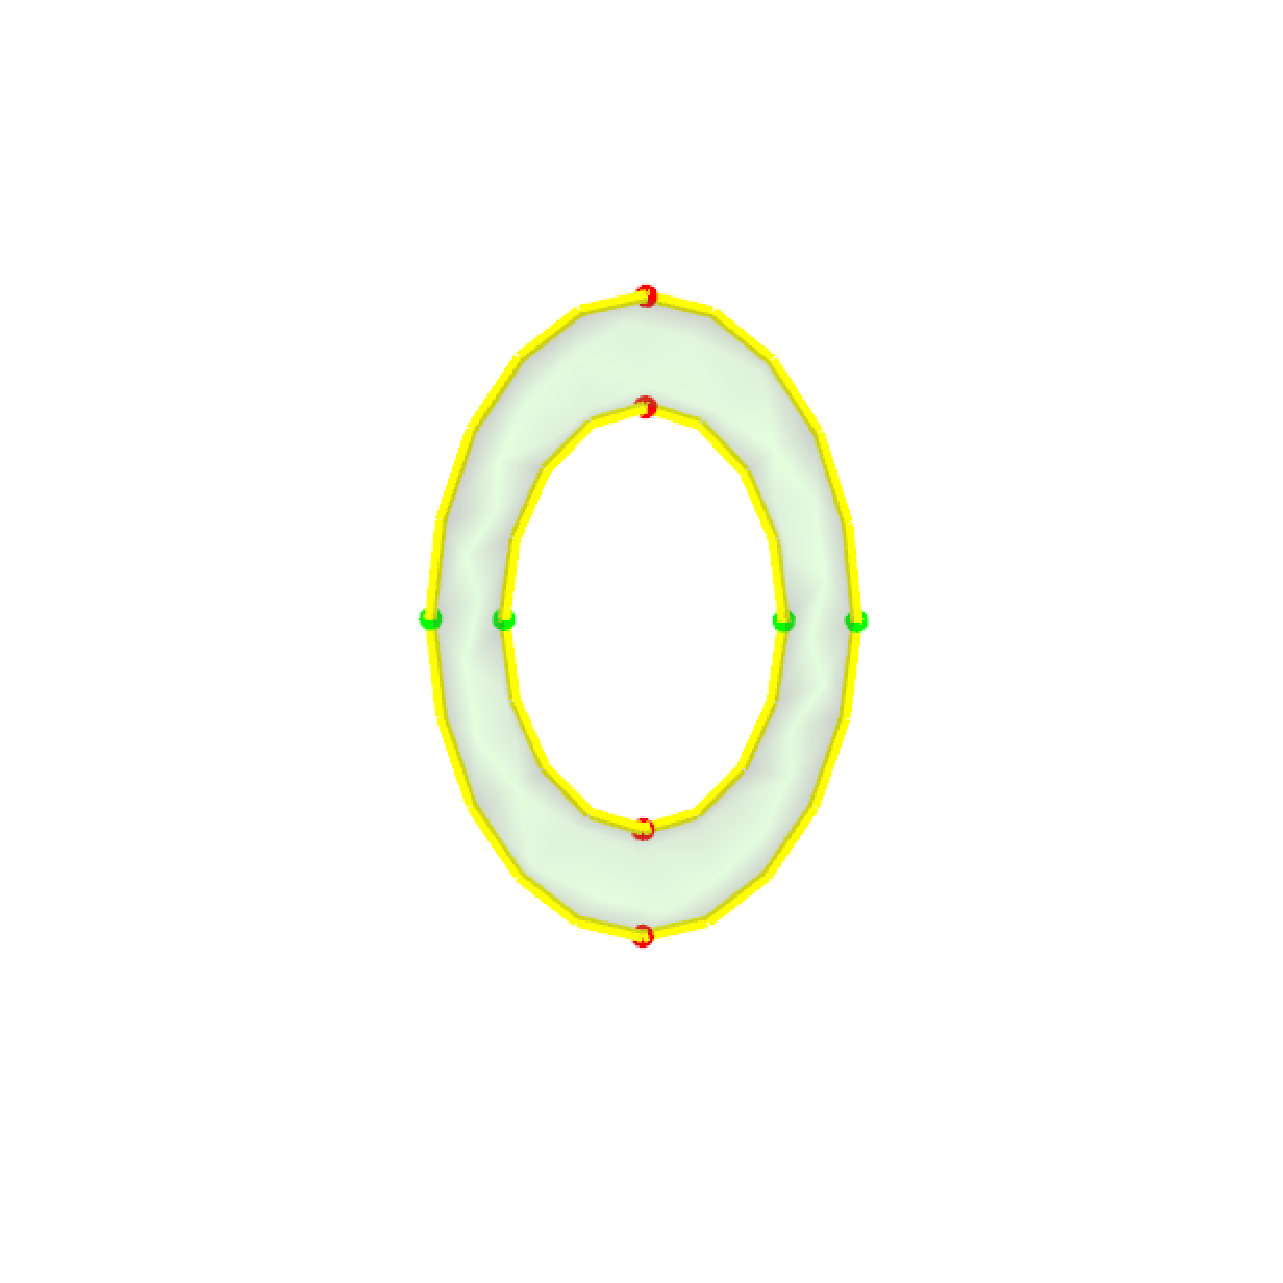
\includegraphics[scale=0.18]{figs/f3.3.3Hole2-2-ps.eps}
    \end{minipage}}
  \subfigure[]{
    \label{fig:uicreationEG:d}
    \begin{minipage}[b]{0.23\textwidth}
      \centering
      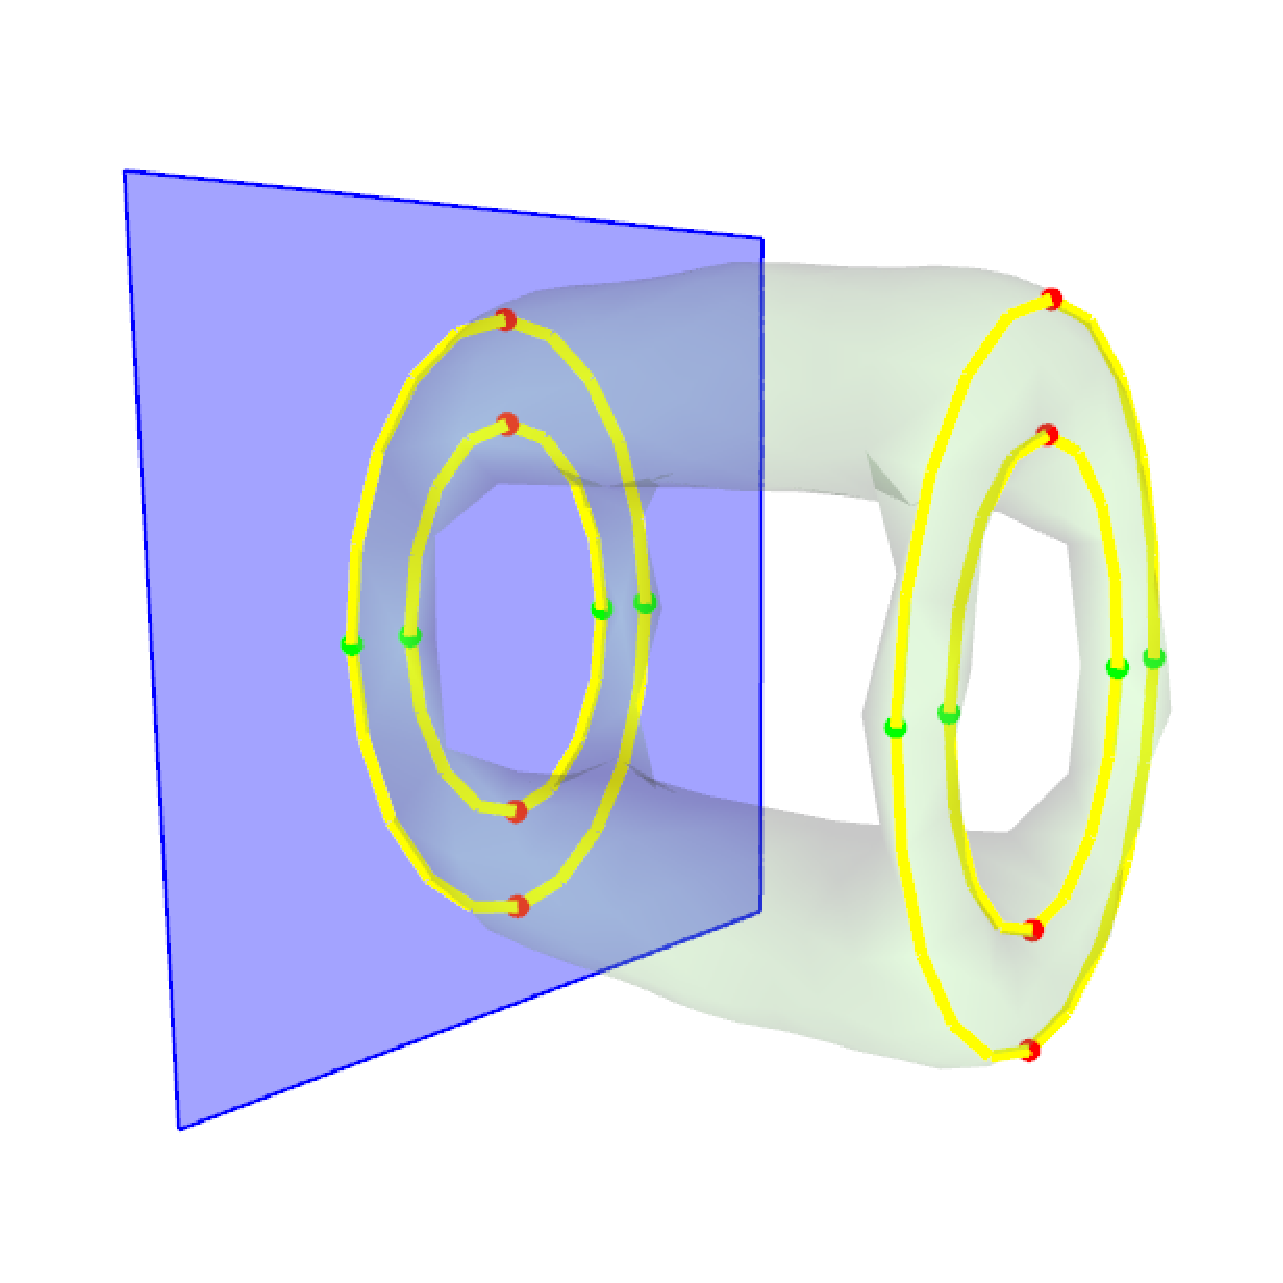
\includegraphics[scale=0.16]{figs/f3.3.3Hole3-1-ps.eps}
    \end{minipage}}
  \subfigure[]{
    \label{fig:uicreationEG:e}
    \begin{minipage}[b]{0.23\textwidth}
      \centering
      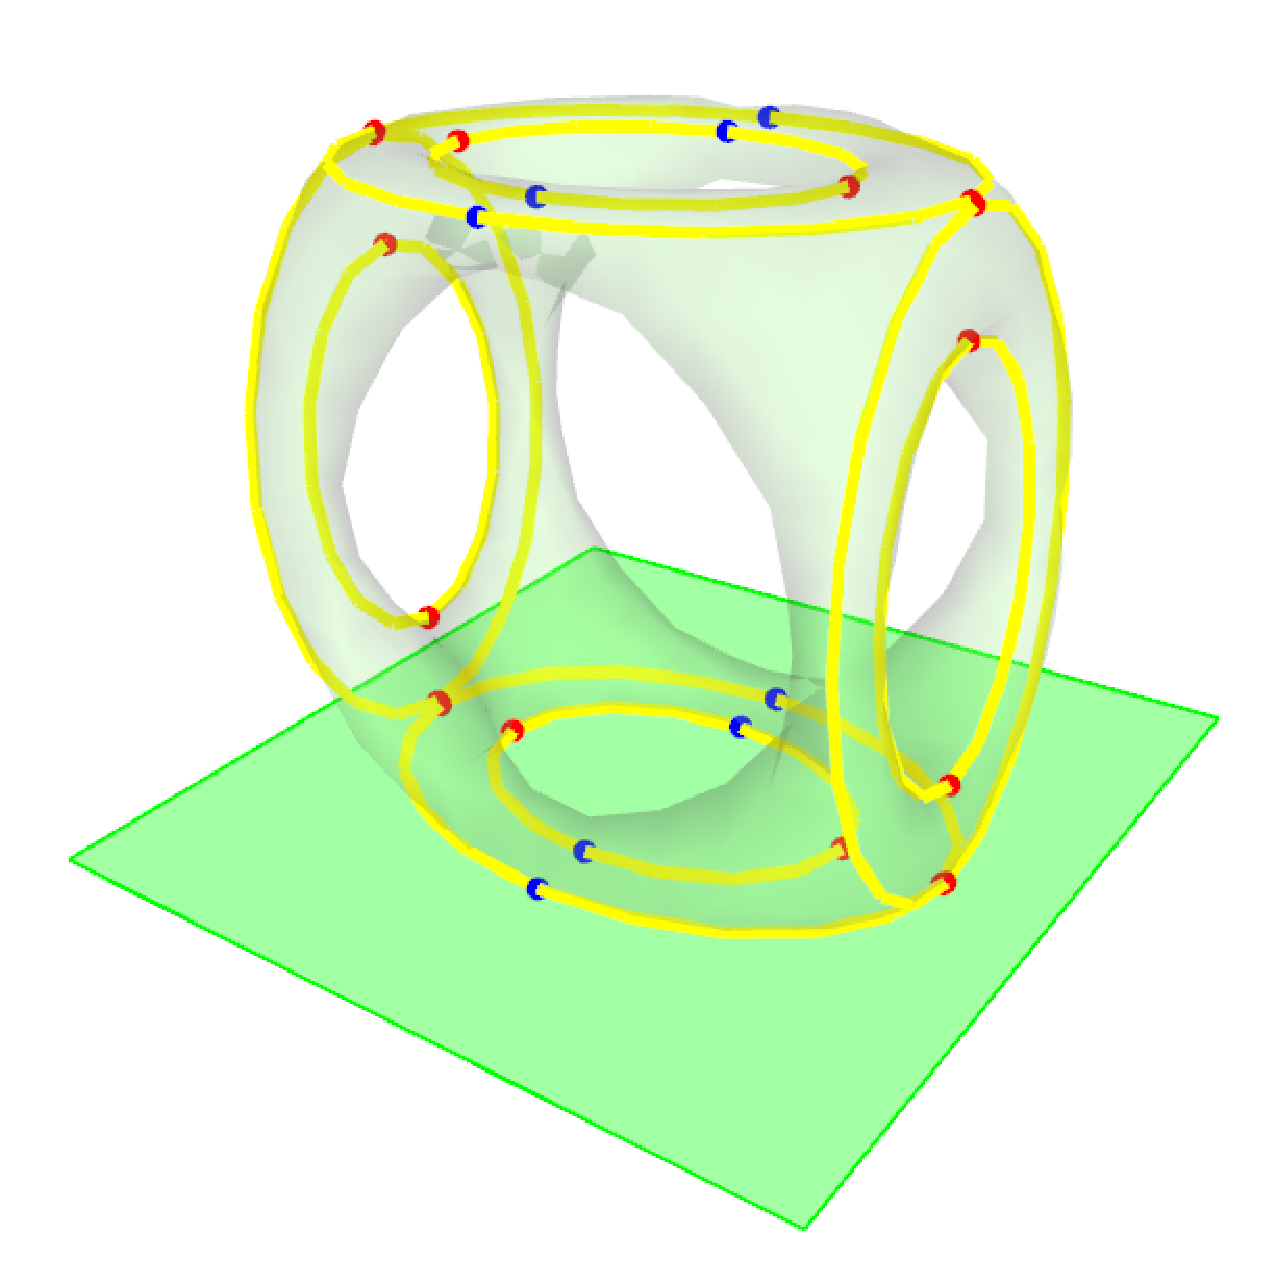
\includegraphics[scale=0.16]{figs/f3.3.3Hole4-1-ps.eps}
    \end{minipage}}
  \subfigure[]{
    \label{fig:uicreationEG:f}
    \begin{minipage}[b]{0.23\textwidth}
      \centering
      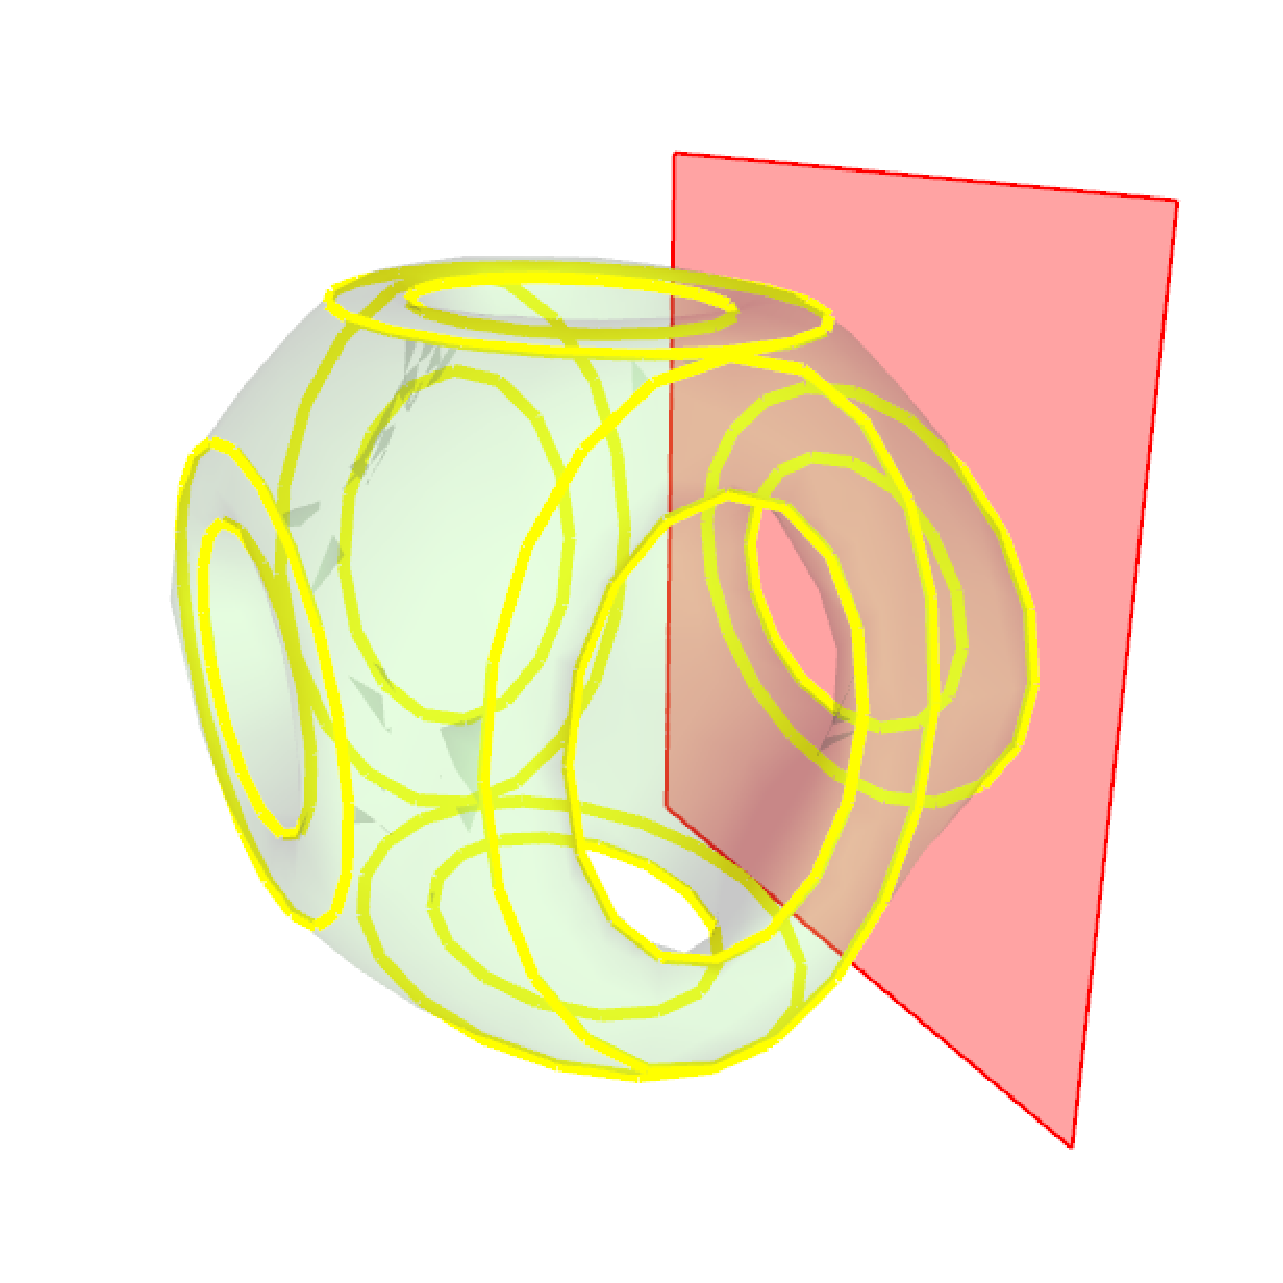
\includegraphics[scale=0.18]{figs/f3.3.3Hole5-1-ps.eps}
    \end{minipage}}
  \subfigure[]{
    \label{fig:uicreationEG:g}
    \begin{minipage}[b]{0.23\textwidth}
      \centering
      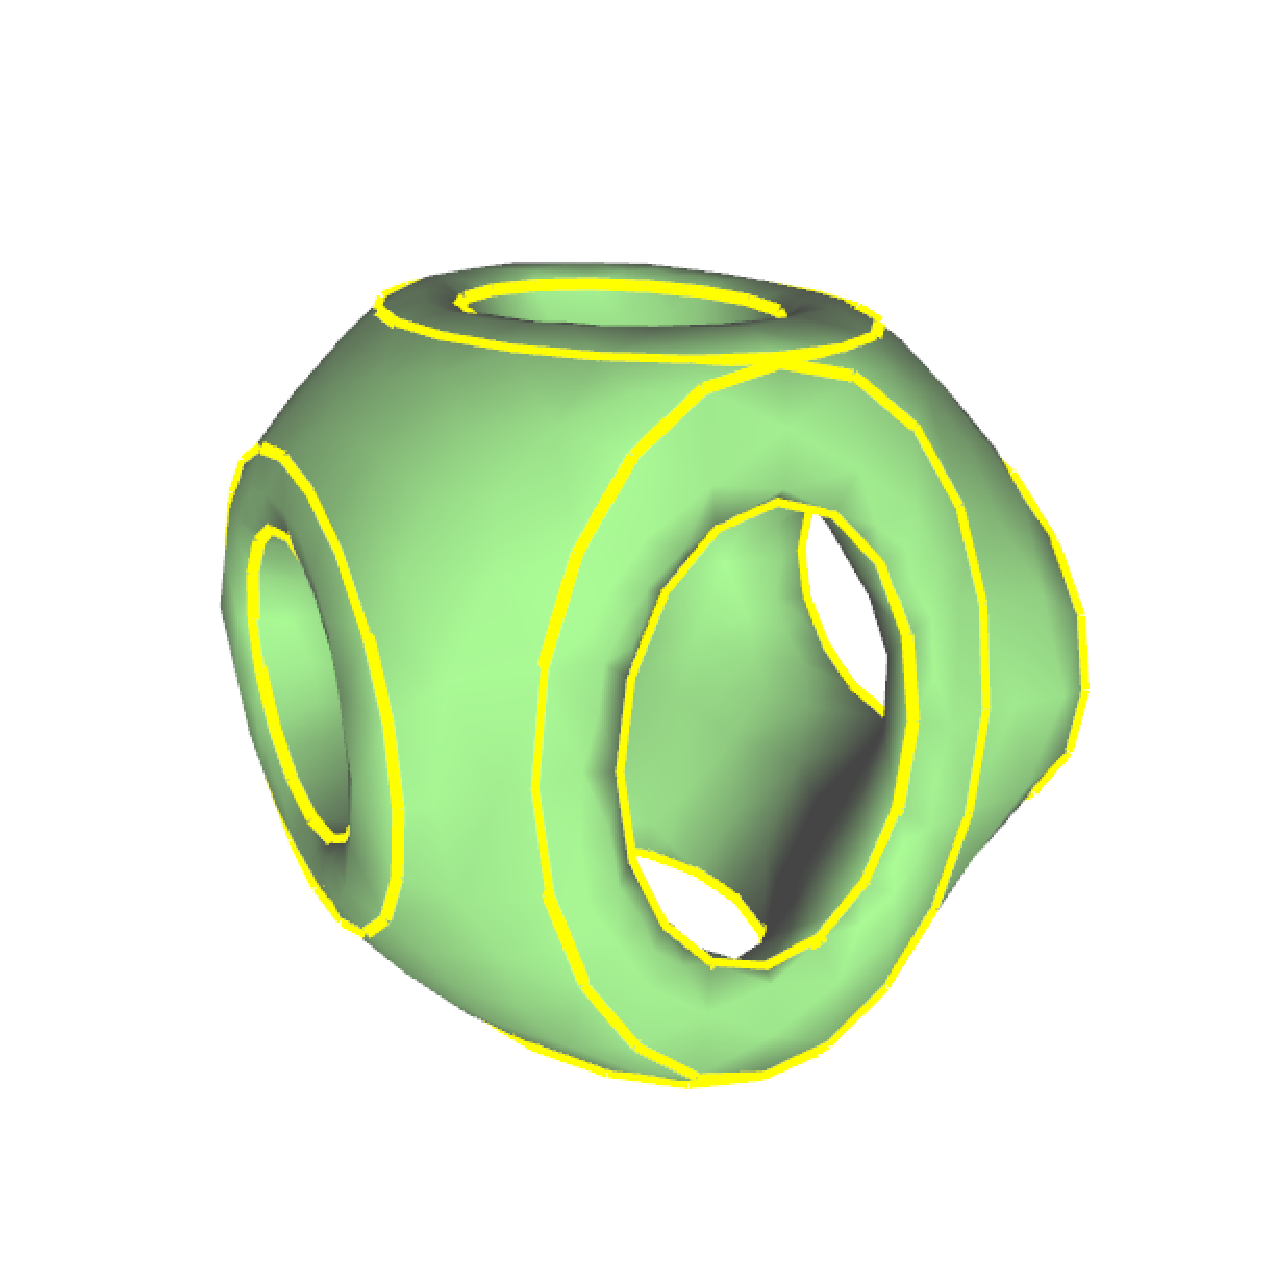
\includegraphics[scale=0.18]{figs/f3.3.3Hole6-ps.eps}
    \end{minipage}}
  \subfigure[]{
    \label{fig:uicreationEG:h}
    \begin{minipage}[b]{0.23\textwidth}
      \centering
      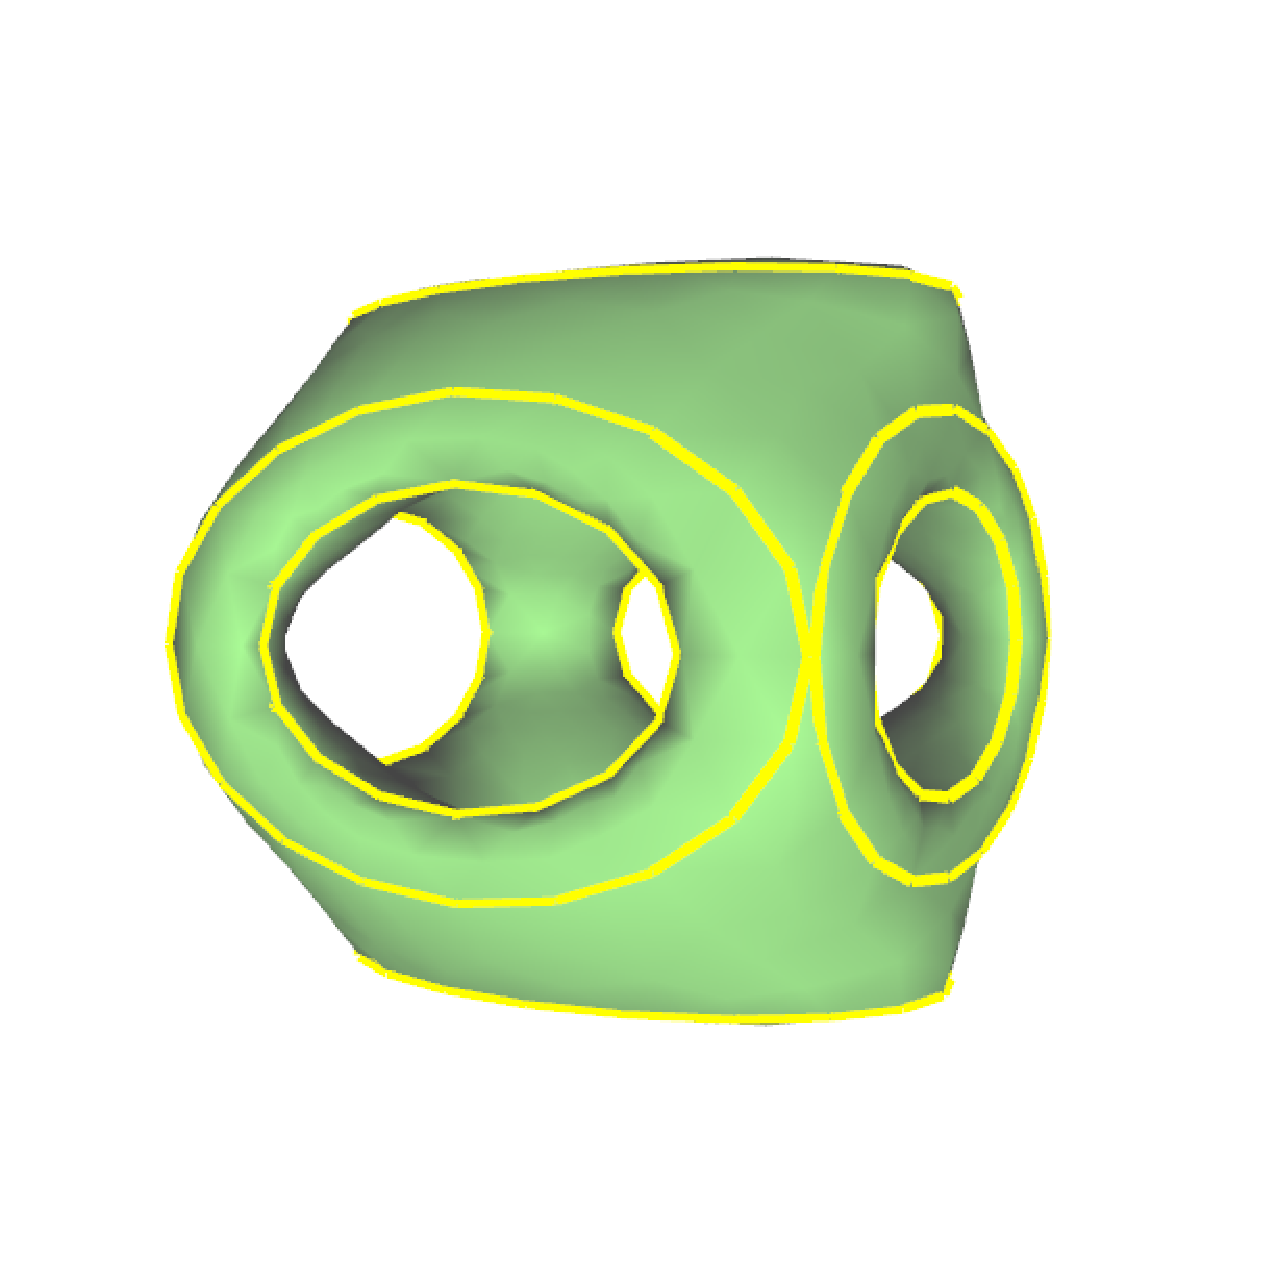
\includegraphics[scale=0.18]{figs/f3.3.3Hole6-1-ps.eps}
    \end{minipage}}
  \caption{An example of using the creation tool. (a) Initially, three basic planes are provided. (b) Two closed curves are sketched on the blue plane. (c) The preview of the current shape reconstructed from the two curves. (d) Another two closed curves are drawn on the translated blue plane and the previewed shape is rendered. (e)-(f) The same operations are performed on the green and red planes. (g)-(h) Two views of the finally generated model.}
  \label{fig:uicreationEG} %% label for entire figure
\end{figure}

These three basic planes can also be translated along $x$, $y$ and $z$ axis respectively to allow the sketch of more contour curves. This can result in several sets of parallel cross section contours. Note that though it is possible to rotate the basic planes to provide more general reference planes and this could give the user more flexibilities to sketch the contours, the price for this flexibility is the algorithmic complexity of constructing 3D models from non-parallel curve networks, the complexity of design and use of interface, and the increase of occurrence of various ambiguities from sketching. Therefore after a careful trade-off, we just allow the basic planes to be translated and we find that this is generally sufficient in practice for sketch-based free-form design.

By manipulating the reference planes, the user can have a direct feel and touch of the 3D space, 3D positions and orientations will thus be more clear and the accuracy of sketching can be enhanced. This makes our method more flexible and intuitive than the fixed multi-view interface in conventional 3D modeling tools. Meanwhile, we render the planes as semi-transparent to avoid blocking the model itself when providing sketching assistance to the user.

%automatic view rotation
It has been observed that a good view for the user to sketch the 2D strokes is the one that has a large visible projection~\cite{BBS08}. So in our system after the user selects a reference plane to sketch on, the view is automatically rotated to make the normal of the plane consistent with the view direction, such that the plane faces the user as much as possible. The system smoothly animates the process of the rotation and the user can terminate it at any time when he feels it is suitable for sketching. This ensures that the view rotation does not disturb the user's focus on designing.

%preview function
Each time the user finishes the sketchings on a plane, the up-to-date model interpolating the cross sections will be reconstructed and rendered transparently upon the user's request. Comparing to the sculpting technique, sketching is an indirect way of communicating with a shape, and it relies on the sense of human perception~\cite{CIW08}. This preview function thus helps the user to get a clear mind of the geometry and relative proportions of the constructed model after each sketch.  It also gives hint and reference on the following sketches and makes the final shape \lq\lq{least surprising}\rq\rq to the user. 
%user study to see whether the user tends to switch it on or off
%here should also mention the conclusion of user study

%sketched and calculated cross sections, highlited intersection points
During the sketching process, all the user sketched cross sections, as well as the calculated cross sections between the previewed model and reference planes, are displayed and can be modified through oversketching or deleted. We also highlighted the intersection points between these cross section curves and the reference planes, such that it will be easy to maintain the coherency of different sketchings for the user. It is noticed that when the preview 
function is  turned on and the calculated cross sections are oversketched, the modeling process is quite similar to that in some existing sketch-based modeling systems~\cite{NISA07,MI07,SWS10}, which allow the user to \lq\lq{sculpt}\rq\rq a model iteratively by modifying handle curves on it. However, in our system the user is free to sketch arbitrary cross section curves in 3D space to depict the shape of the model, which is more similar to the sketching behavior in real world and thus the modeling will be more flexible and convenient.

Figure~\ref{fig:uicreationEG} shows an overview of the creation process. With the help of the three sets of reference planes, more descriptions on the shape of a model can be sketched. This speeds up the production process of a 3D model.

It should be pointed out that even though the reference planes are useful for defining the shape of a model, sometimes ambiguity still occurs. The ambiguity arises from two aspects: the user input strokes may not necessarily follow the same style -- different users may have different manners for defining the shape of a model; even with the same contours, the understandings of the shape they defined may vary among different users. So some rules must be provided for sketching the contours. The details of the rules will be discussed in Chapter~\ref{ch3:sec:alg:creation}.


%-----------------------------------------------------------------------------------------------------------------
\subsection{Sculpting Tool}\label{ch3:sec:ui:sculpt}

After the user sketches the general shape of the model, we provide a series of sculpting functions, to allow the further refinement. The sculpting tools include the deformation, extrusion, tunneling (digging a hole), cutting and smoothing functions, all of which are based on user sketches. An intelligent stroke recognition mechanism is used to judge the user's intention according to the sketches and switch to the corresponding sculpting tool automatically.

\subsubsection{Stroke Recognition}\label{ch3:sec:ui:StrReco}

\begin{figure} [htbp]
  \centering
  \subfigure[]{
    \centering
    \label{fig:uicutting} %% label for first subfigure
    \begin{minipage}[b]{0.5\textwidth}
      \centering
      \includegraphics[scale=0.11]{figs/f3.CuttingEG.eps}
    \end{minipage}}
   \subfigure[]{
    \centering
    \label{fig:uismoothing} %% label for first subfigure
    \begin{minipage}[b]{0.4\textwidth}
      \centering
      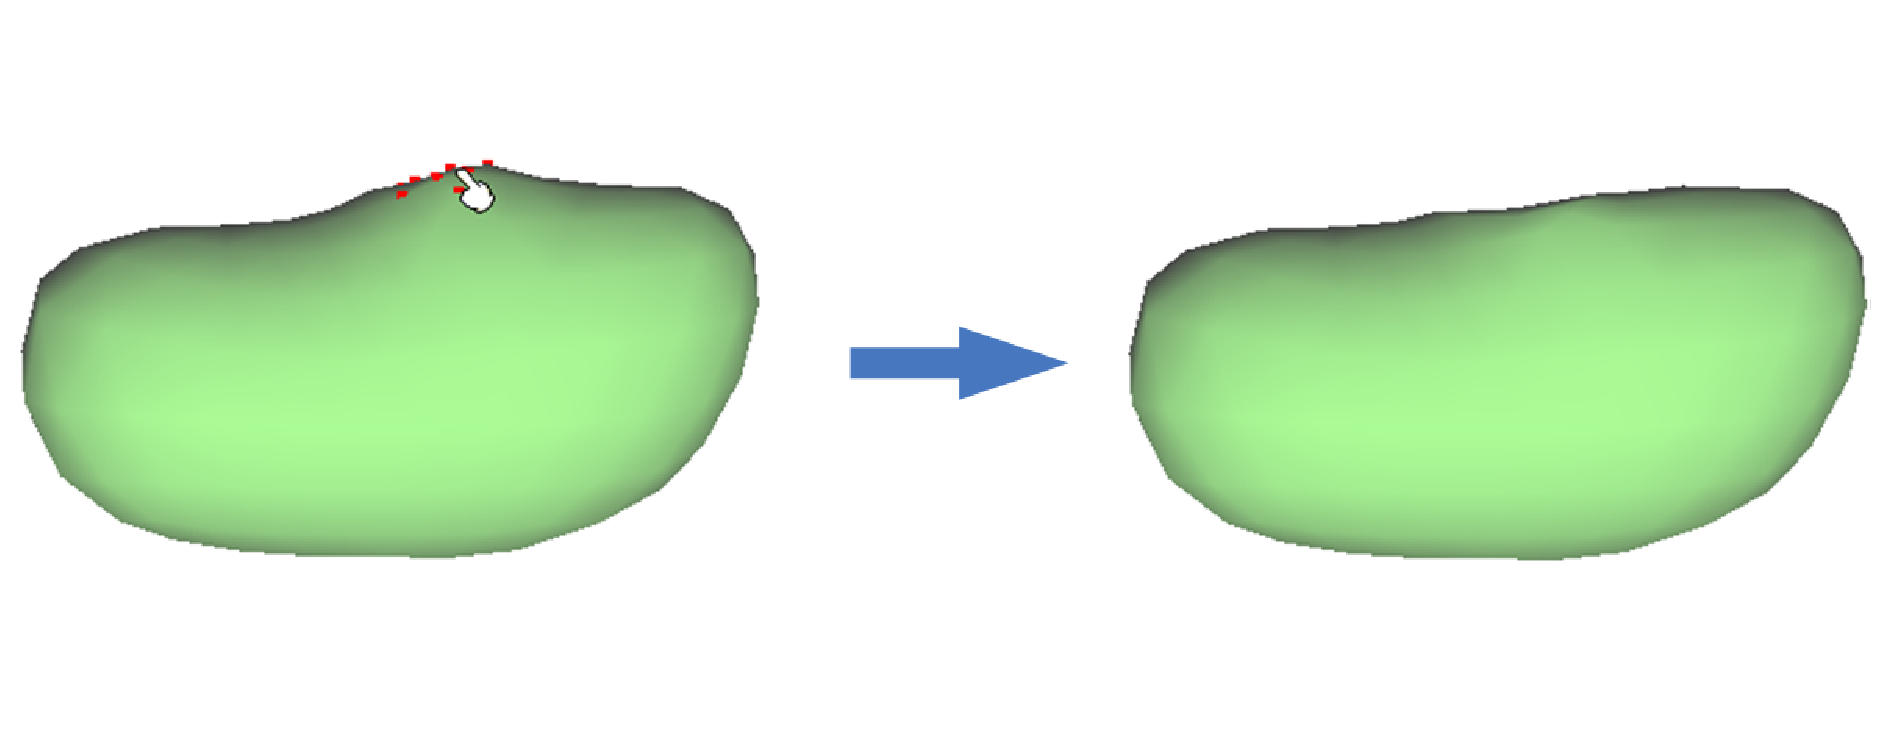
\includegraphics[scale=0.16]{figs/f3.SmoothingEG.eps}
    \end{minipage}}
  \caption{(a) Cutting operation. (b) Smoothing operation.}
  \label{fig:uicuttingsmoothing} %% label for entire figure
\end{figure}

\begin{figure} [htbp]
  \centering
  \subfigure[]{
    \centering
    \label{fig:uiextrusion} %% label for first subfigure
    \begin{minipage}[b]{0.8\textwidth}
      \centering
      \includegraphics[scale=0.2]{figs/f3.extrusion.eps}
    \end{minipage}}
  \\
   \subfigure[]{
    \centering
    \label{fig:uitunneling} %% label for first subfigure
    \begin{minipage}[b]{0.8\textwidth}
      \centering
      \includegraphics[scale=0.18]{figs/f3.tunneling.eps}
    \end{minipage}}
  \caption{(a) Extrusion operation. (b) Tunneling operation.}
  \label{fig:uiextrusiontunneling} %% label for entire figure
\end{figure}


The stroke set our system accepts in the sculpting tool include three general types: a simple open stroke, a closed stroke, and a scratch-out stroke. When a simple open stroke is sketched, the operation may be cutting or deformation, depending on whether the stroke has passed across the model in image space or not. If it is a cutting stroke, a following stroke will be required to indicate which part to cut off (Figure~\ref{fig:uicutting}). The subsequent operation of deformation will be introduced in detail in~\ref{ch3:sec:ui:deformation}.

We allow the user to extrude or dig a part similar to the operation in~\cite{IMT99,NISA07} when a closed stroke is sketched on the surface of the model. What is different, our system automatically generates a reference plane orthogonal to the closed curve, on which the user can draw the silhouette curve of the extruded/dug part (Figure~\ref{fig:uiextrusion}). This plane could be rotated about two axes: the line passing through the center of the 
closed stroke and orthogonal to the stroke as much as possible or the line connecting the first drawn point of the closed stroke and the farthest point to it on the stroke. The reference plane helps to confirm the position of the silhouette curve and gives flexibility to adjust its direction. When the silhouette curve intersects with the backside surface, the operation turns to tunneling and a hole is dug (Figure~\ref{fig:uitunneling}). 

When the user scratch a part on the model back and forth, it is regarded as a smoothing operation and the local part will be smoothed (Figure~\ref{fig:uismoothing}).


\subsubsection{Deformation Tool}\label{ch3:sec:ui:deformation}

The deformation tool is an important sculpting function in our system. To deform a mesh, the user needs to sketch a stroke which will be projected onto the mesh, generating a handle curve. Two reference planes will be generated automatically. The user then needs to sketch on the reference planes to specify the new shape and position of the handle curve, after which the deformation is completed. To implement this deformation process, the following information should be specified: a set of vertices (called handle vertices) and their new positions; the vertices within a region of interest (ROI), which will move with the handles; and the vertices will remain unchanged during the deformation process (called the static vertices).

To generate the handle curve, we use a method similar to that in~\cite{NSAC05}. The handle curve is composed of handle vertices. The vertices of the edges or faces on which the projection of the input stroke lie are regarded as the handle vertices. See Figure~\ref{fig:uideformhandle:b} for an example.

\begin{figure} [htbp]
  \centering
  \subfigure[]{
    \centering
    \label{fig:uideformhandle:a} %% label for first subfigure
    \begin{minipage}[b]{0.2\textwidth}
      \centering
      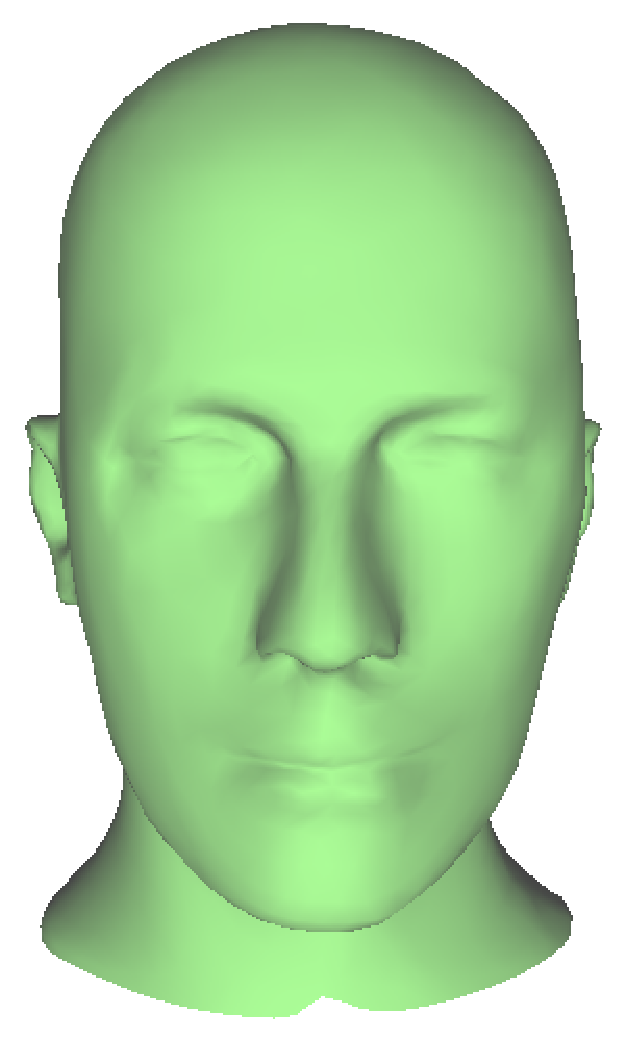
\includegraphics[scale=0.15]{figs/f3.4.a.eps}
    \end{minipage}}
  \subfigure[]{
    \centering
    \label{fig:uideformhandle:b}
    \begin{minipage}[b]{0.2\textwidth}
      \centering
      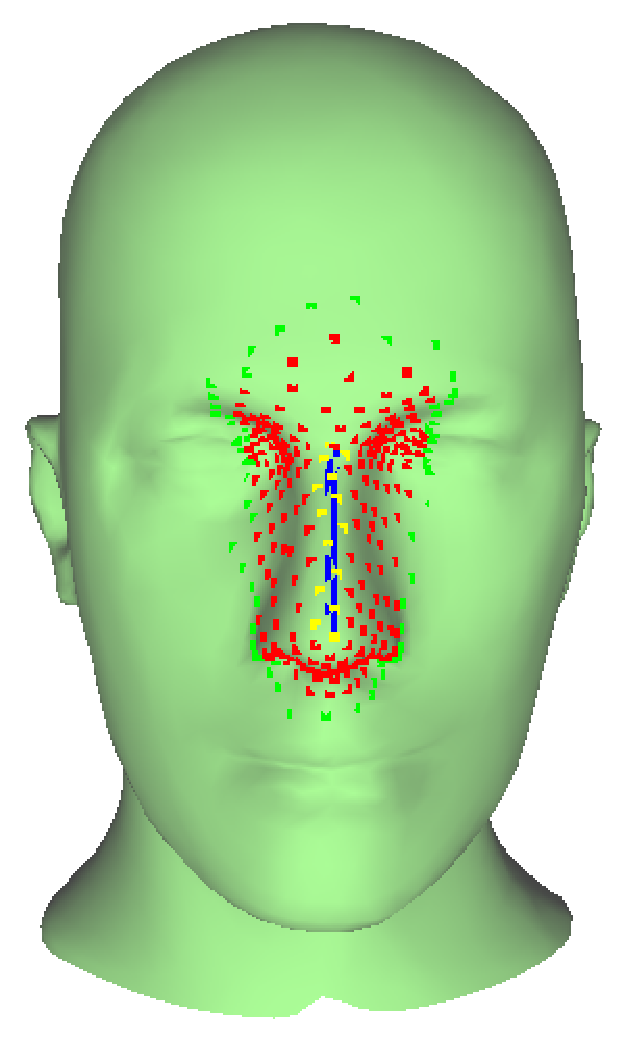
\includegraphics[scale=0.15]{figs/f3.4.b.eps}
    \end{minipage}}
  \subfigure[]{
    \centering
    \label{fig:uideformhandle:c}
    \begin{minipage}[b]{0.23\textwidth}
      \centering
      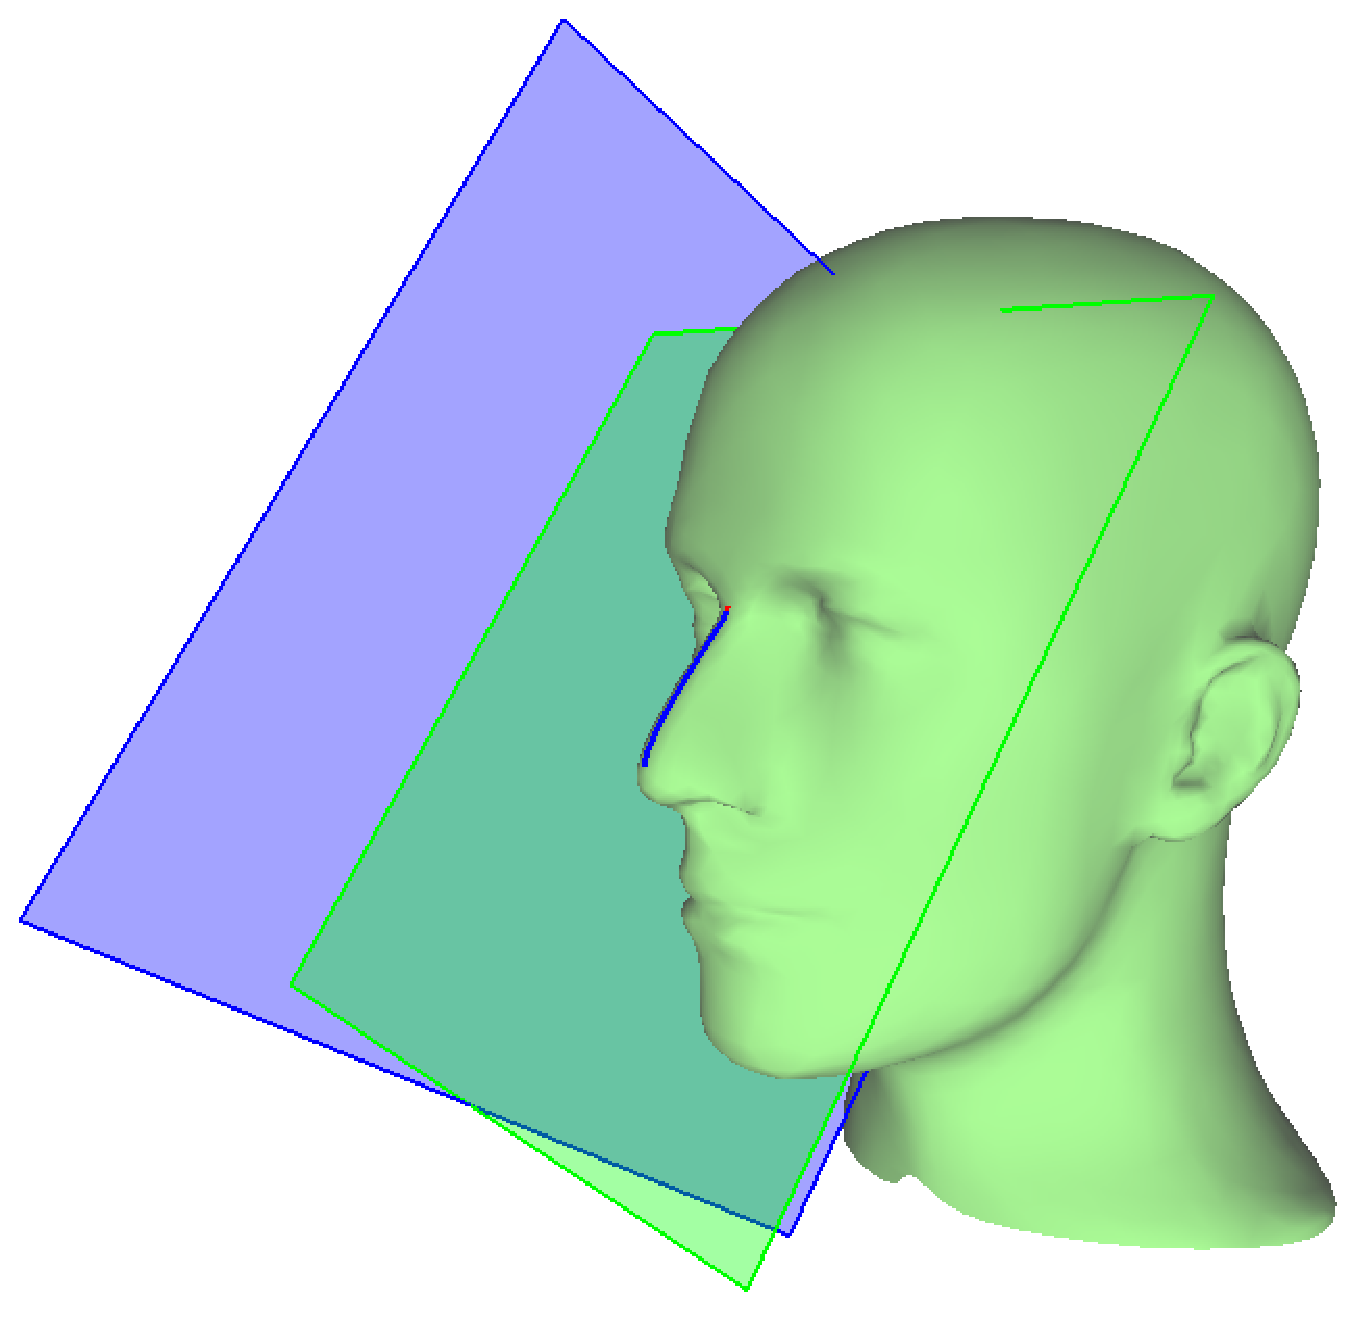
\includegraphics[scale=0.15]{figs/f3.4.c.eps}
    \end{minipage}}
  \subfigure[]{
    \label{fig:uideformhandle:d}
    \begin{minipage}[b]{0.26\textwidth}
      \centering
      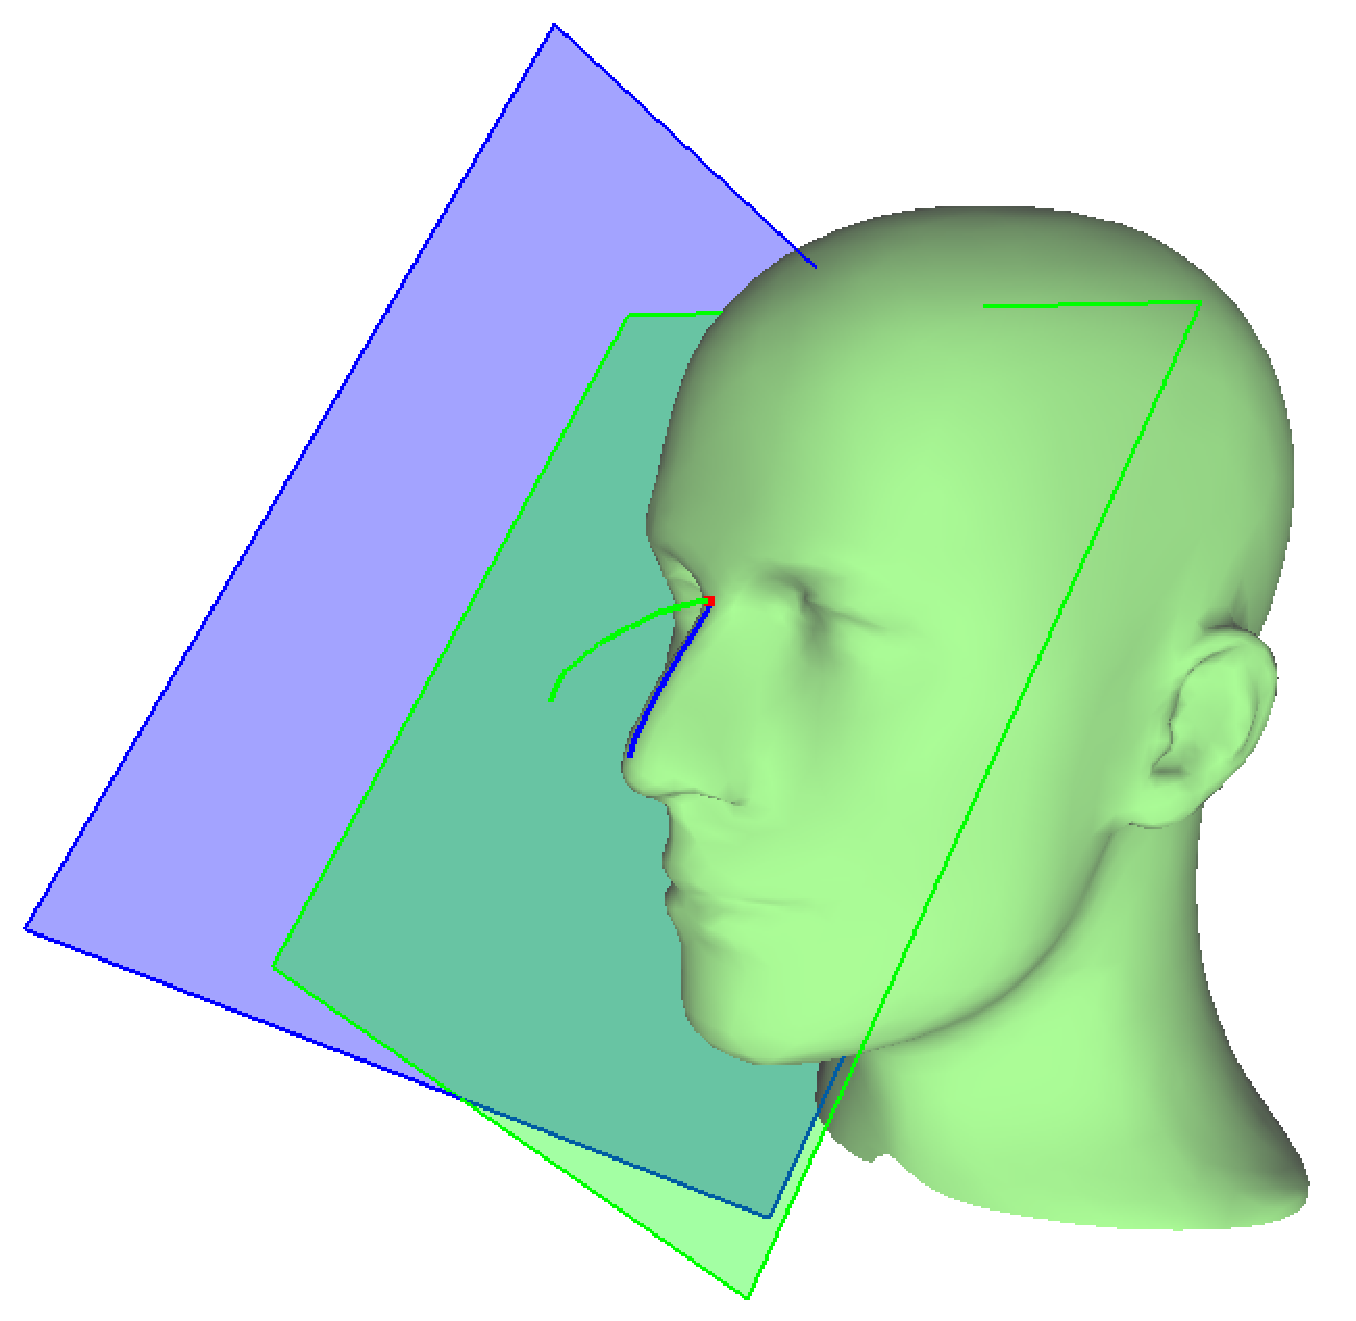
\includegraphics[scale=0.15]{figs/f3.4.d.eps}
    \end{minipage}}
    \\
  \subfigure[]{
    \label{fig:uideformhandle:e}
    \begin{minipage}[b]{0.23\textwidth}
      \centering
      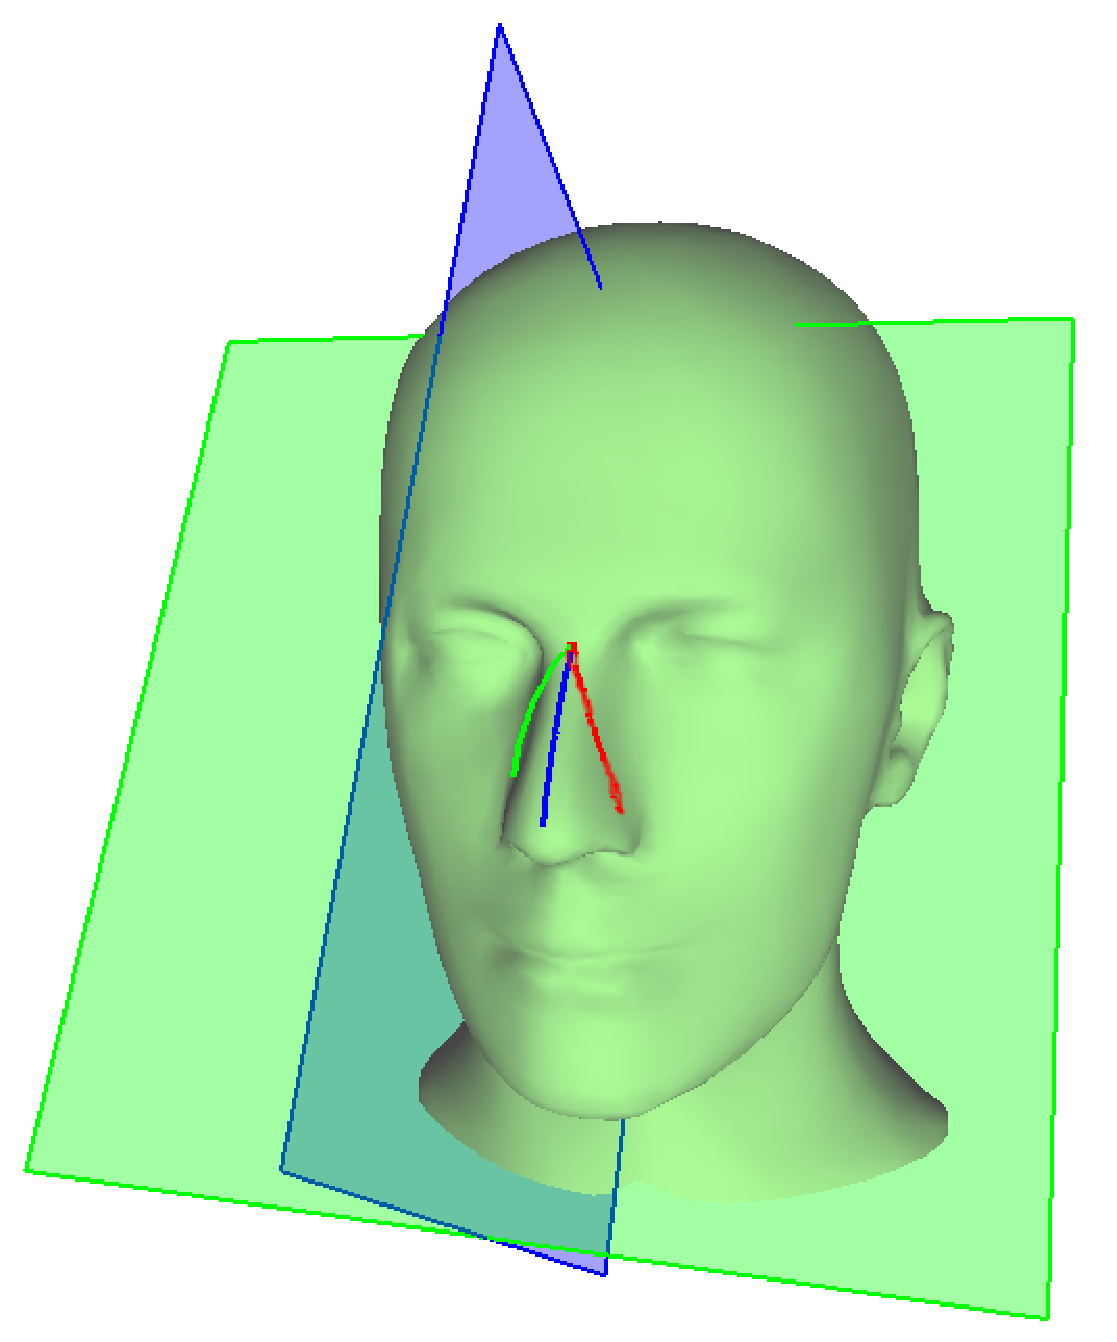
\includegraphics[scale=0.15]{figs/f3.4.e.eps}
    \end{minipage}}
  \subfigure[]{
    \label{fig:uideformhandle:f}
    \begin{minipage}[b]{0.23\textwidth}
      \centering
      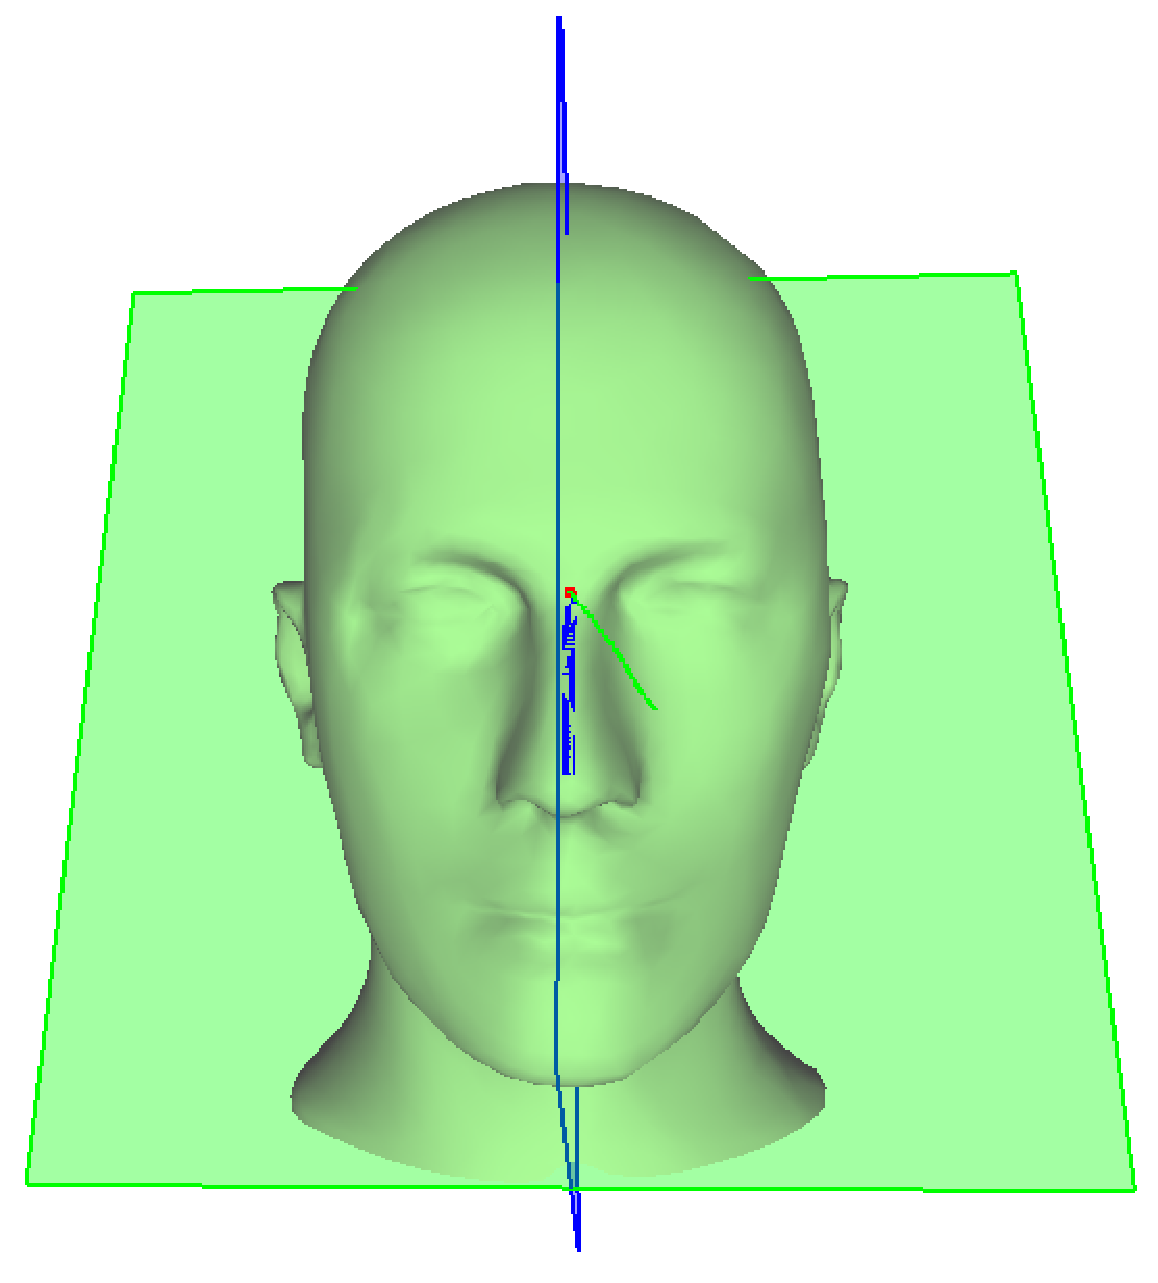
\includegraphics[scale=0.15]{figs/f3.4.f.eps}
    \end{minipage}}
  \subfigure[]{
    \label{fig:uideformhandle:g}
    \begin{minipage}[b]{0.23\textwidth}
      \centering
      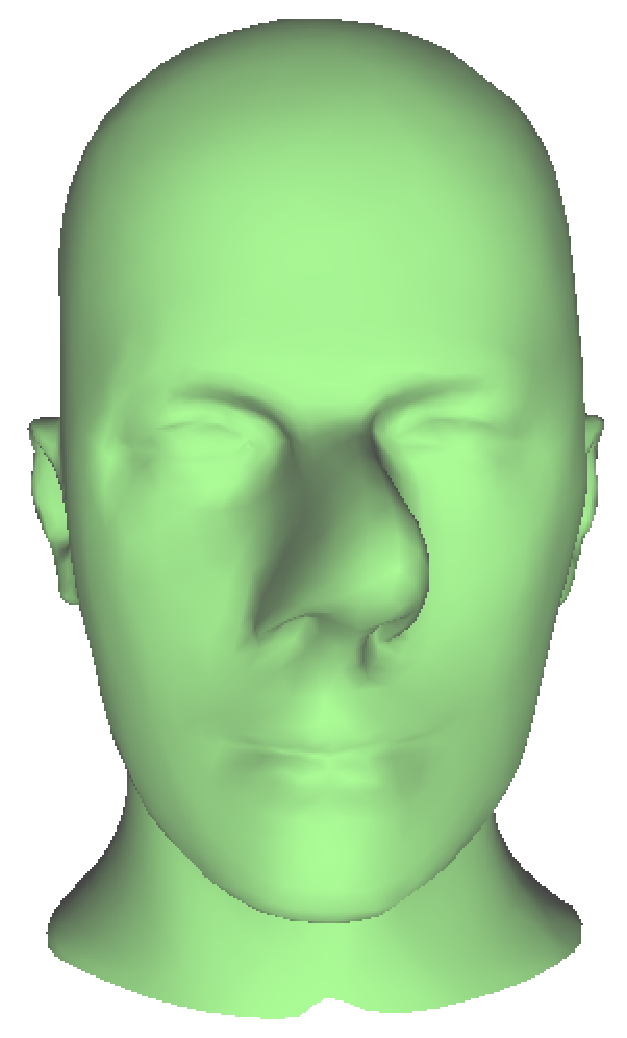
\includegraphics[scale=0.15]{figs/f3.4.g.eps}
    \end{minipage}}
  \caption{An example of using the deformation tool. (a) The initial model. (b) The blue curve on the mesh is the handle curve projected from a 2D user sketch. The yellow, red and green dots denote the handle, ROI and static vertices respectively. (c) The generated base plane (blue) and projection plane (green). (d) The new curve (green) drawn on the base plane. (e) A curve (red) is drawn in the projection plane to create a non-planar new curve. (f) The updated new curve (green). (g) The deformed model.}
  \label{fig:uideformhandle} %% label for entire figure
\end{figure}

The specification of new positions of the handle vertices seems not trivial. Unlike previous existing methods, we provide the user with two reference planes for the sketching of the new curve: a base plane which passes the handle vertices as many as possible for sketching the basic shape of the new curve and a projection plane, which is orthogonal to the base plane, for drawing the projection of the new curve (see Figure~\ref{fig:uideformhandle:c}). In general, the base plane is sufficient for sketching the new shape of the handle curve. However, if the new handle curve is desired to be non-planar, the projection plane is used to sketch its projection(Figure~\ref{fig:uideformhandle:d} - Figure~\ref{fig:uideformhandle:f}) and then the new handle curve is determined. In addition, in our system the two planes can also be rotated to provide more flexibility. In this way, the user can draw arbitrary curves in 3D space while being fully aware of the locations.

For selection of the ROI vertices, three methods are available. A simple approach is to specify a threshold and vertices whose Euclidean distances to the handles below this threshold are regarded as the ROI vertices. Another approach is to let user draw a circle on the 2D screen. The ROI vertices are the ones whose projections onto the screen are inside the circle. However these two methods seem not quite precise when the selection of certain vertices is required for relatively complex models. So we provide a new tool -- a brush, to make the selection process somewhat like brushing on a model. The vertices brushed will then be chosen as the ROI vertices. The brush can be viewed as a complementary tool for the former two methods. The user could take a rough selection using the first two tools and then make further modifications by brushing on the model.

These sculpting tools are all sketch-based and quite convenient to use. Together with the creation function, a complete modeling system is built up. With this system, the user could easily create and edit a 3D object in a short period by sketching strokes. An example for the whole process of producing a 3D model is in Figure~\ref{fig:uichair}.

\begin{figure} [htbp]
  \centering
  \subfigure[]{
    \centering
    \label{fig:uichair:a} %% label for first subfigure
    \begin{minipage}[b]{0.16\textwidth}
      \centering
      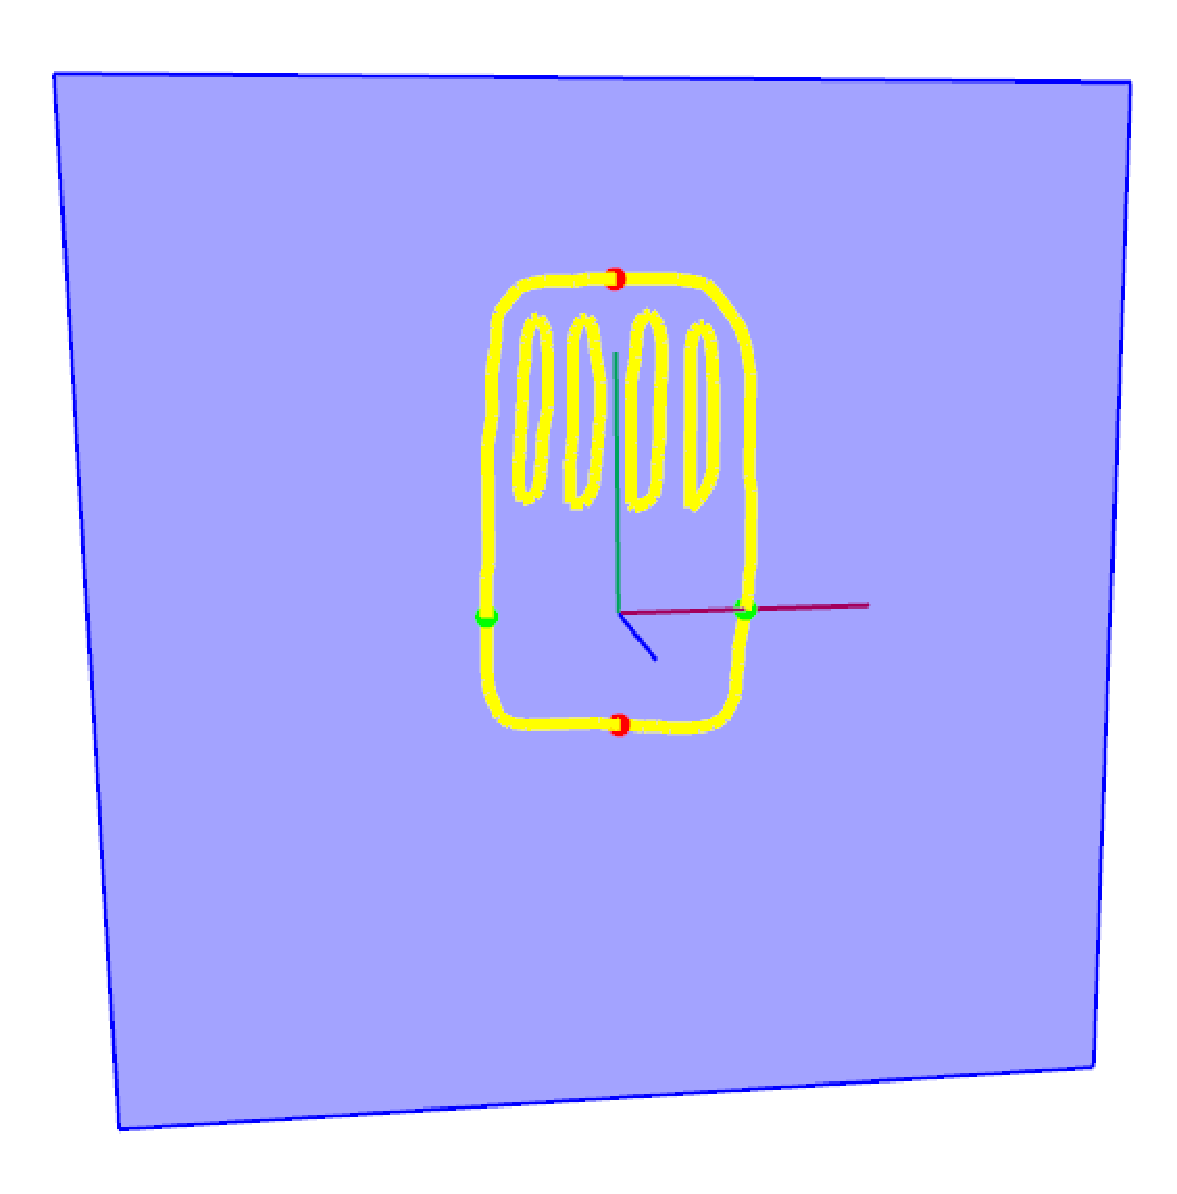
\includegraphics[scale=0.14]{figs/f3.chair1.eps}
    \end{minipage}}
  \subfigure[]{
    \centering
    \label{fig:uichair:b}
    \begin{minipage}[b]{0.16\textwidth}
      \centering
      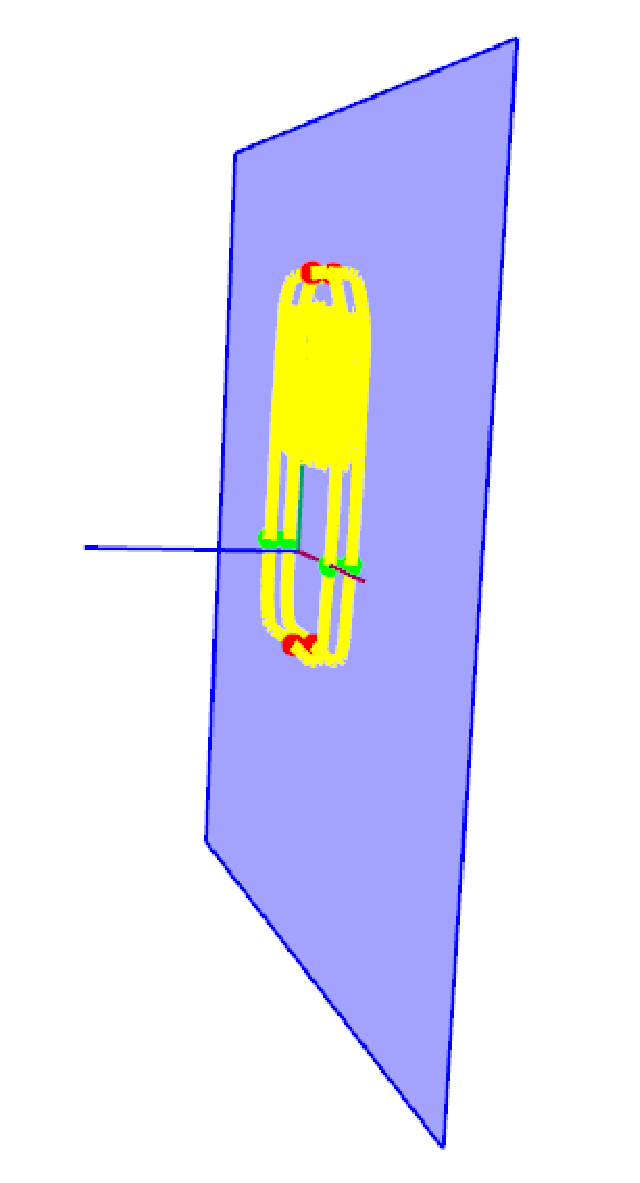
\includegraphics[scale=0.14]{figs/f3.chair2.eps}
    \end{minipage}}
  \subfigure[]{
    \centering
    \label{fig:uichair:c}
    \begin{minipage}[b]{0.16\textwidth}
      \centering
      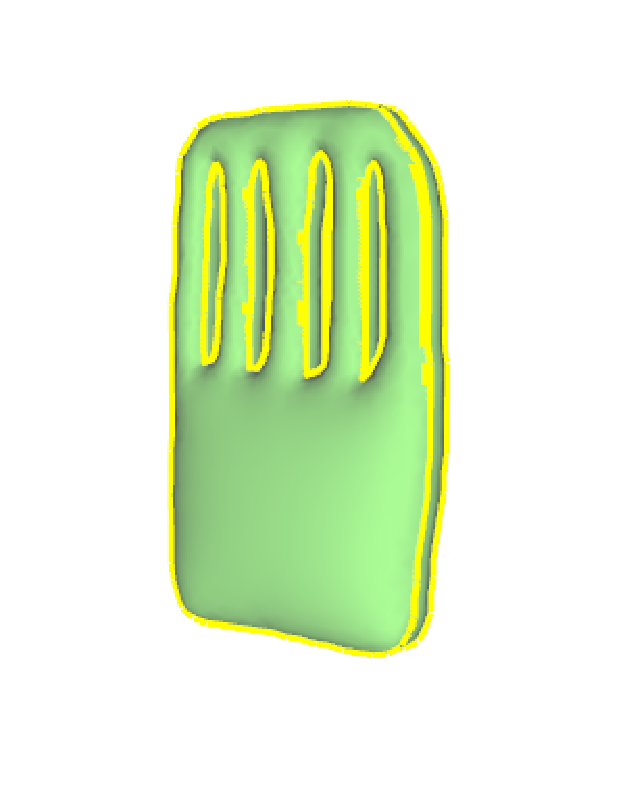
\includegraphics[scale=0.22]{figs/f3.chair3.eps}
    \end{minipage}}
  \subfigure[]{
    \label{fig:uichair:d}
    \begin{minipage}[b]{0.20\textwidth}
      \centering
      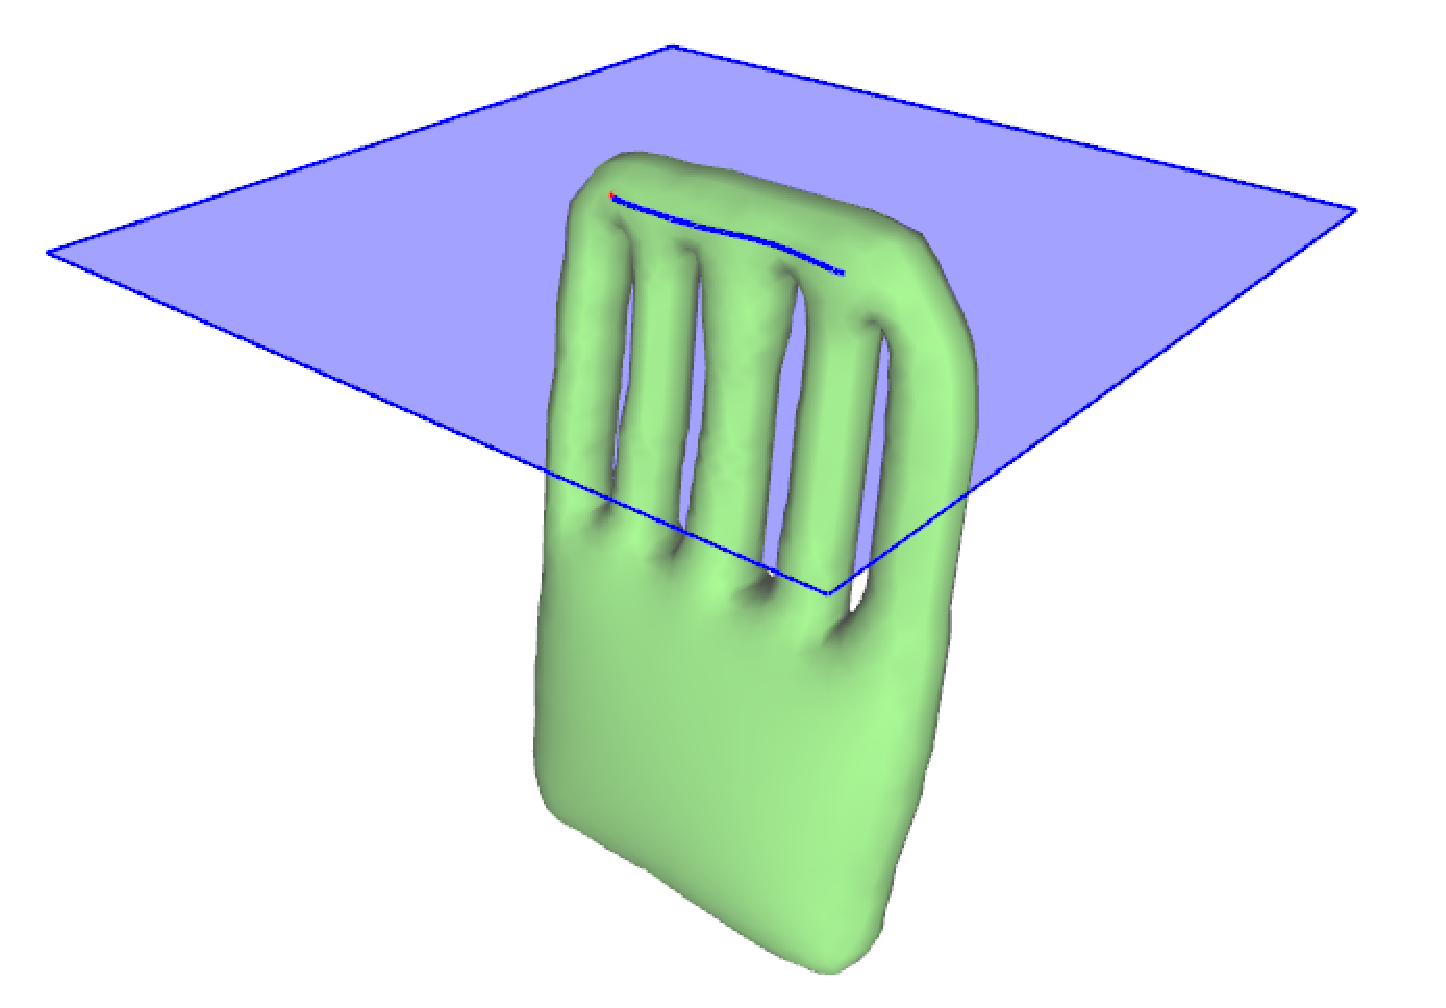
\includegraphics[scale=0.12]{figs/f3.chair4.eps}
    \end{minipage}}
  \subfigure[]{
    \label{fig:uichair:e}
    \begin{minipage}[b]{0.16\textwidth}
      \centering
      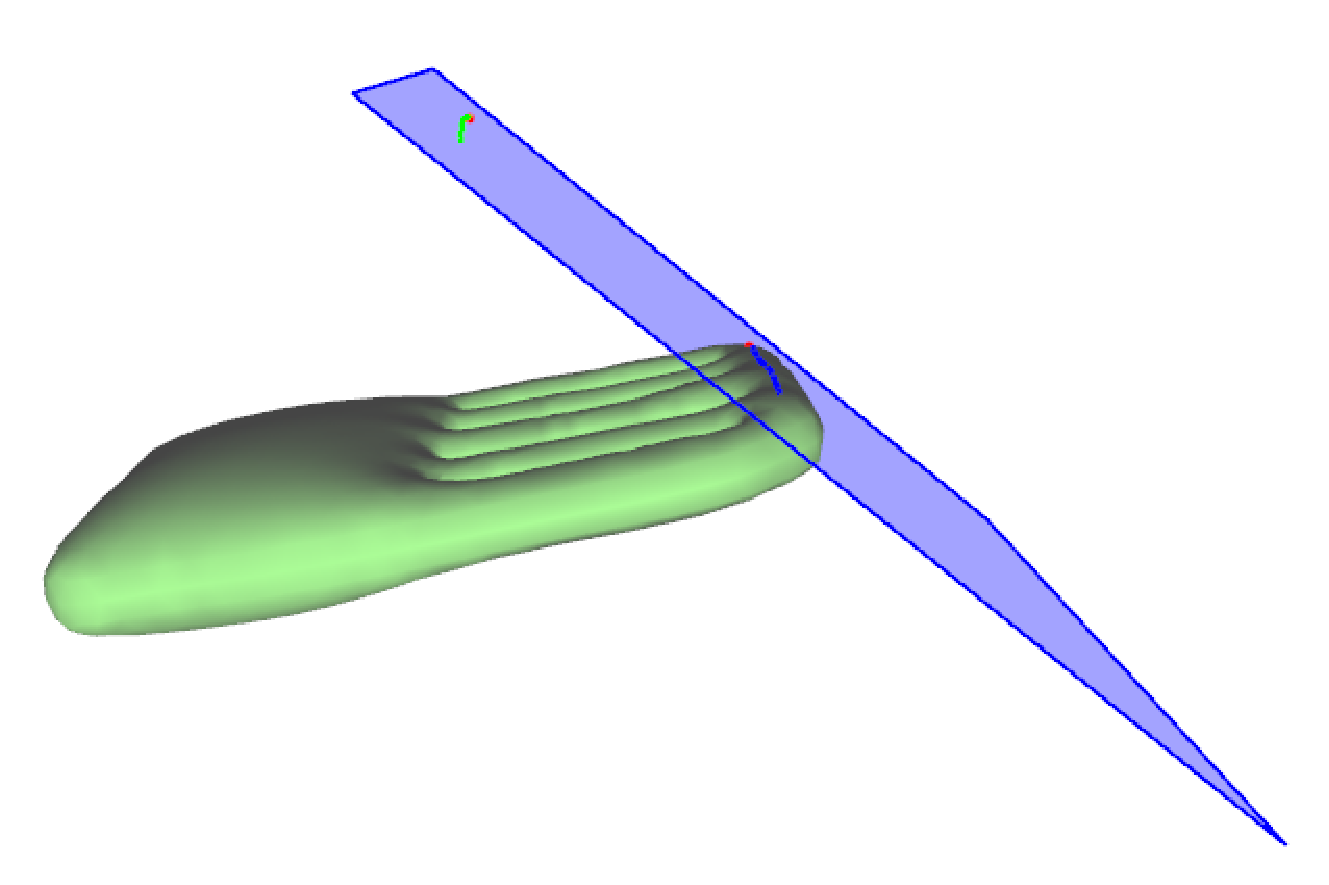
\includegraphics[scale=0.14]{figs/f3.chair5.eps}
    \end{minipage}}
    \\
  \subfigure[]{
    \label{fig:uichair:f}
    \begin{minipage}[b]{0.16\textwidth}
      \centering
      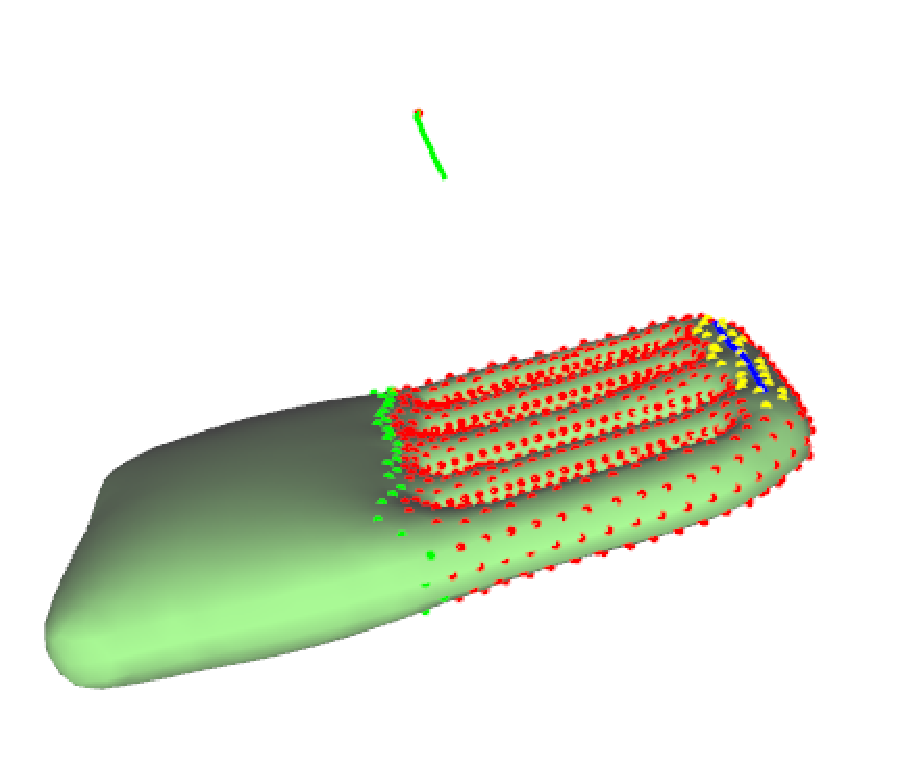
\includegraphics[scale=0.14]{figs/f3.chair6.eps}
    \end{minipage}}
  \subfigure[]{
    \label{fig:uichair:g}
    \begin{minipage}[b]{0.18\textwidth}
      \centering
      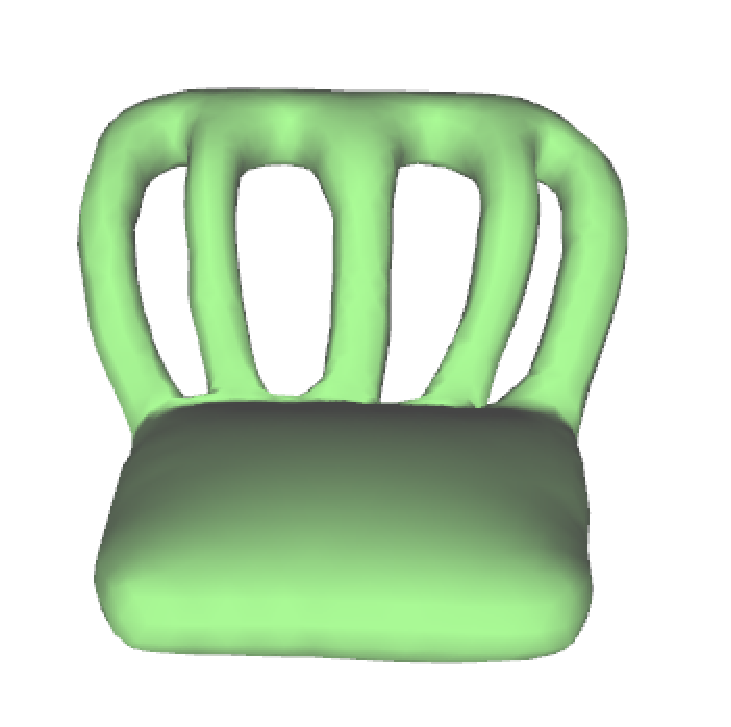
\includegraphics[scale=0.16]{figs/f3.chair7.eps}
    \end{minipage}}
  \subfigure[]{
    \label{fig:uichair:h}
    \begin{minipage}[b]{0.18\textwidth}
      \centering
      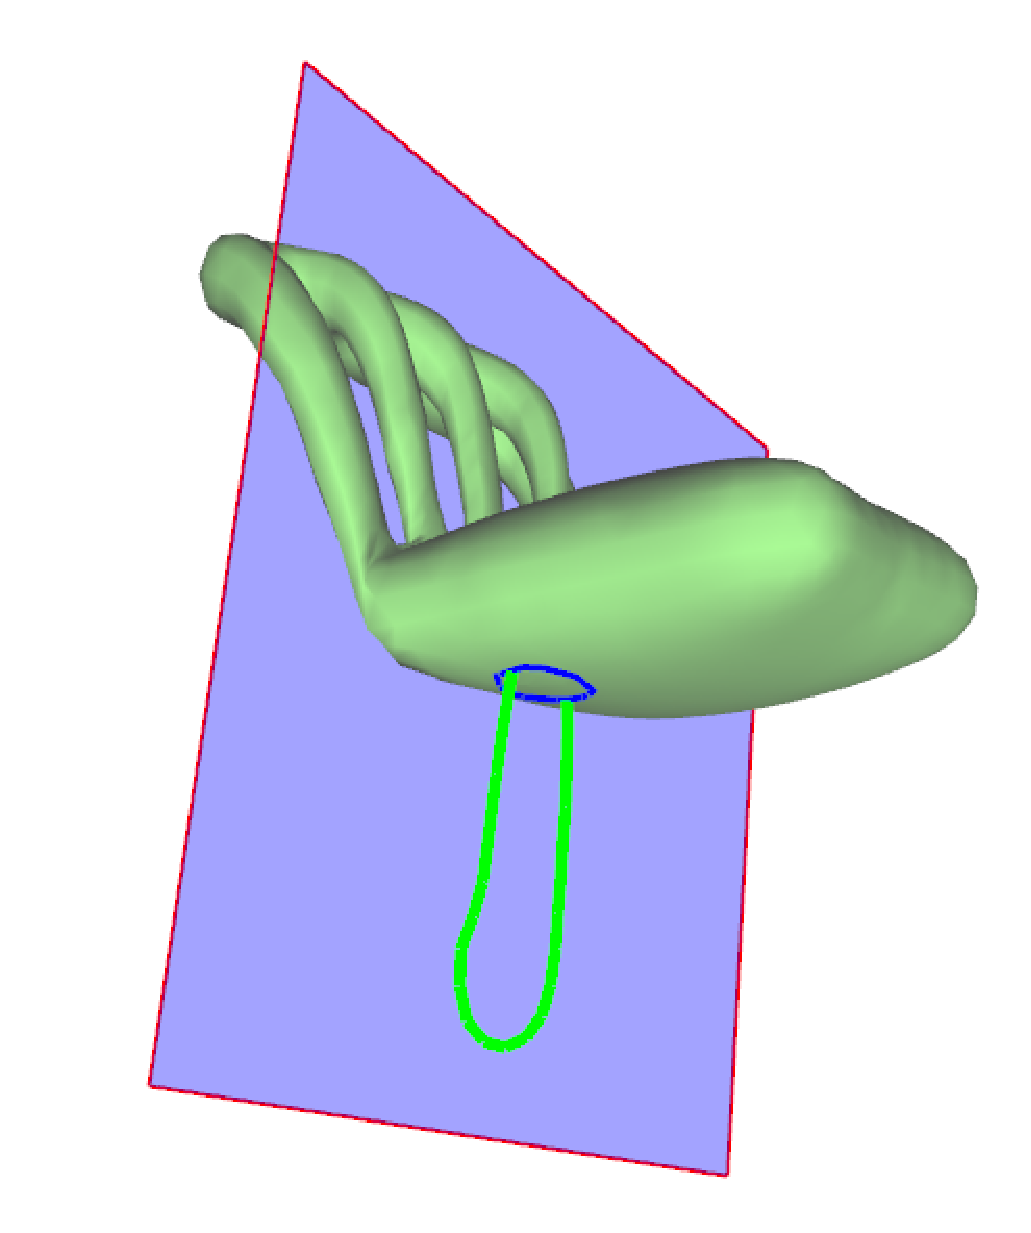
\includegraphics[scale=0.14]{figs/f3.chair8.eps}
    \end{minipage}}
  \subfigure[]{
    \label{fig:uichair:i}
    \begin{minipage}[b]{0.18\textwidth}
      \centering
      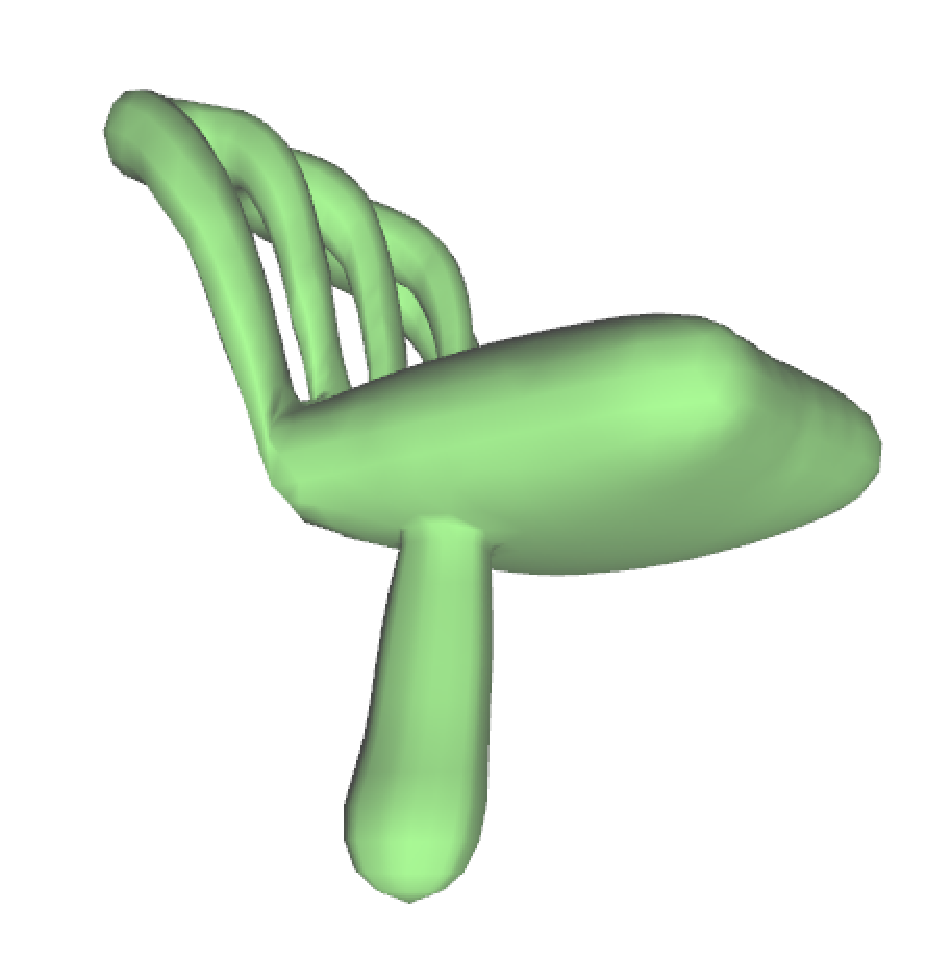
\includegraphics[scale=0.14]{figs/f3.chair9.eps}
    \end{minipage}}
  \subfigure[]{
    \label{fig:uichair:j}
    \begin{minipage}[b]{0.22\textwidth}
      \centering
      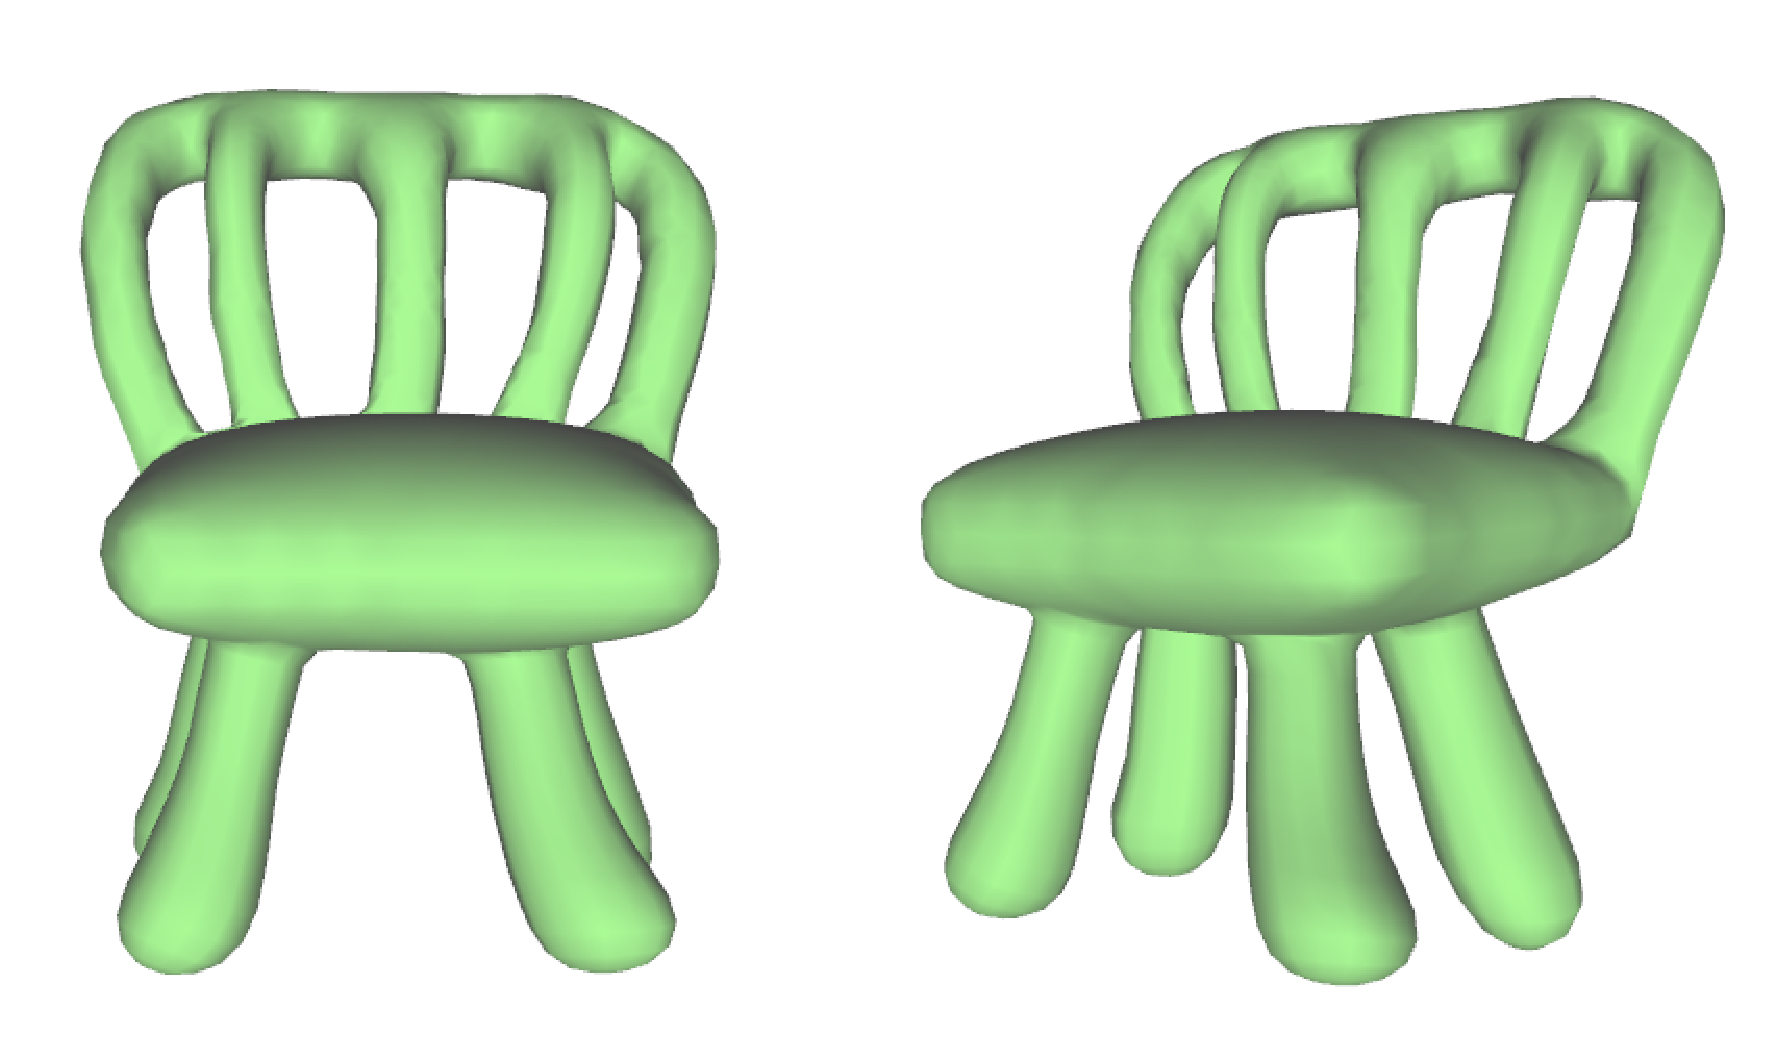
\includegraphics[scale=0.14]{figs/f3.chair10.eps}
    \end{minipage}}
  \caption{An example of modeling using our system. (a)-(c) Creation. (d)-(g) Deformation. (h)-(i) Extrusion. (j) Final result.}
  \label{fig:uichair} %% label for entire figure
\end{figure}

%-----------------------------------------------------------------------------------------------------------------
\section{Algorithm}\label{ch3:sec:alg}

We now introduce the underlying algorithms for the sketching interface, including the stroke preprocessing, the surface reconstruction from 2D sketches, the mesh deformation and the subsequent local refinement, and other related algorithms.

%-----------------------------------------------------------------------------------------------------------------
\subsection{Input Stroke Preprocessing}\label{ch3:sec:alg:strokepreproc}

For sketch-based modeling systems, the original input stroke created from an input device usually cannot be used directly due to several reasons. First, the points of the stroke are noisy because of the shaky nature of handling the input devices. In addition, the spatial and temporal quantization of the input by the hardware may contain error since the speed that the user draws is random. Thus, we perform a three-step preprocessing of the input stroke in each functions, as shown in Figure~\ref{fig:alstrokeproc}.

\begin{figure} [htbp]
  \centering
  \subfigure[]{
    \centering
    \label{fig:alstrokeproc:a} %% label for first subfigure
    \begin{minipage}[b]{0.2\textwidth}
      \centering
      \includegraphics[scale=0.3]{figs/f3.9.a.eps}
    \end{minipage}}
  \subfigure[]{
    \centering
    \label{fig:alstrokeproc:b}
    \begin{minipage}[b]{0.2\textwidth}
      \centering
      \includegraphics[scale=0.3]{figs/f3.9.b.eps}
    \end{minipage}}
  \subfigure[]{
    \centering
    \label{fig:alstrokeproc:c}
    \begin{minipage}[b]{0.2\textwidth}
      \centering
      \includegraphics[scale=0.3]{figs/f3.9.c.eps}
    \end{minipage}}
  \subfigure[]{
    \centering
    \label{fig:alstrokeproc:d}
    \begin{minipage}[b]{0.2\textwidth}
      \centering
      \includegraphics[scale=0.3]{figs/f3.9.d.eps}
    \end{minipage}}
  \caption{Stroke Preprocessing: The goal here is to filter the noisy points and get a smooth curve with 10 points. (a) Initial input. (b) Filtering result. (c) Resampling result. (d) Final result after smoothing.}
  \label{fig:alstrokeproc} %% label for entire figure
\end{figure}

First of all, a point whose distance to its previous one is less than a given threshold will be judged as a redundant noisy point and deleted.

Then we resample the stroke to make its points number a predefined value $N_{pre}$. To do this, we first calculate the summed distance $S_{total}$ between each two points to get the length of the stroke. Then through dividing $S_{total}$ by $N_{pre}$, we get the expected unit distance $S_{unit}=S_{total} / N_{pre}$ along the route of the stroke between each two new points. Finally starting from the first point, we \lq\lq{travel}\rq\rq along the original stroke trajectory. Every time when a unit distance $S_{unit}$ reaches, we position a new stroke point. The \lq\lq{journey}\rq\rq ends until the last new point is placed. A new curve is then formed.

This simple resample algorithm can produce a stroke with desired number of points. The original shape of the stroke is preserved as much as possible. Meanwhile, it is quite easy to implement and avoids the complicated computations in other methods(for example, fitting a polyline to a B-spline and evenly sample it~\cite{CMZHB99}).

Finally the stroke is smoothed by moving each point according to Eqn~\ref{eq:strokesmooth}.

\begin{equation}
\label{eq:strokesmooth}
	P_i^\prime = \frac{P_{i-1}+4*P_i+P_{i+1}}{6}
\end{equation}

Here $P_i$ and $P_i^\prime$ are the old and new positions of point $i$. $P_{i-1}$ and $P_{i+1}$ are the old positions of its two neighbor points.

The stroke preprocessing is a fundamental step for the functions in the system and helps to produce a visually-pleasant 3D model.

%cross section completion from small strokes, oversketching will be added here

%-----------------------------------------------------------------------------------------------------------------
\subsection{Surface Reconstruction}\label{ch3:sec:alg:creation}

As mentioned earlier, some rules are needed to regularize and interpret the user sketched strokes before we construct the surface. Considering both the widely recognized meaning of the cross section strokes and the human psychology, the following rules are proposed:

\begin{enumerate}
	\item For curves on a plane, if they do not intersect with or contain in each other, the interior of each curve belongs to the interior of the model.
	\label{rule:1}
	\item For two curves $S_1$ and $S_2$ on a plane, if $S_1$ is totally contained in $S_2$, then it means that the intersection between the plane and the model is a ring. If the containing relationship exists among more than two curves, that is, we have $n$ curves $S_1,S_2,...,S_n$ and $S_i$ is within $S_{i+1}$, then we start the perception from the outermost pair of curves $S_n$ and $S_{n-1}$.
	\label{rule:2}
	\item If a curve is self-intersected or intersects with any other curves lying on the same
plane, then it is treated as an invalid curve and thus discarded.
	\label{rule:3}
	\item For two curves $S_1$ and $S_2$ lying on two orthogonal planes $P_1$ and $P_2$ respectively, the intersection point set $\{V_{S_1P_2}\}$ of curve $S_1$ and plane $P_2$, must be exactly the \emph{same} as the set $\{V_{S_2P_1}\}$ of $S_2$ and plane $P_1$.
	\label{rule:4}
\end{enumerate}

Next we give some explanations of these rules. The first rule is easy to understand. When a user draws one or more closed strokes, the strokes are usually regarded as the outer contours of an object.

When a user tries to make a hole on the mesh surface to create a relatively complex model, a pair of curves are often used, of which one is contained in the other. The ring between the two curves is the interior part of the model. If more holes are desired, more pairs of curves should be used. To avoid the ambiguity of perception, the order of analysis is inward starting from the outermost pair. For example, suppose we have $n$ curves $S_1,S_2,...,S_n$ and $S_{i-1}$ is totally contained in  $S_i$. Then $S_n$ and $S_{n-1}$ form a ring, $S_{n-2}$ and $S_{n-3}$ form another ring which is contained in the previous one, and so on. If $n$ is an even number, then the ring formed by $S_2$ and $S_1$ is innermost; Otherwise we just apply rule~\ref{rule:1} to $S_1$ -- the interior of $S_1$ is the interior of the model. An example of rule~\ref{rule:2} is shown in Figure~\ref{fig:rule2}. Rule~\ref{rule:2} makes it possible to model a mesh with arbitrary topology directly by sketching the contours at the creation phase.

\begin{figure} [htbp]
  \centering
  \subfigure[]{
    \centering
    \label{fig:rule2:a} %% label for first subfigure
    \begin{minipage}[b]{0.22\textwidth}
      \centering
      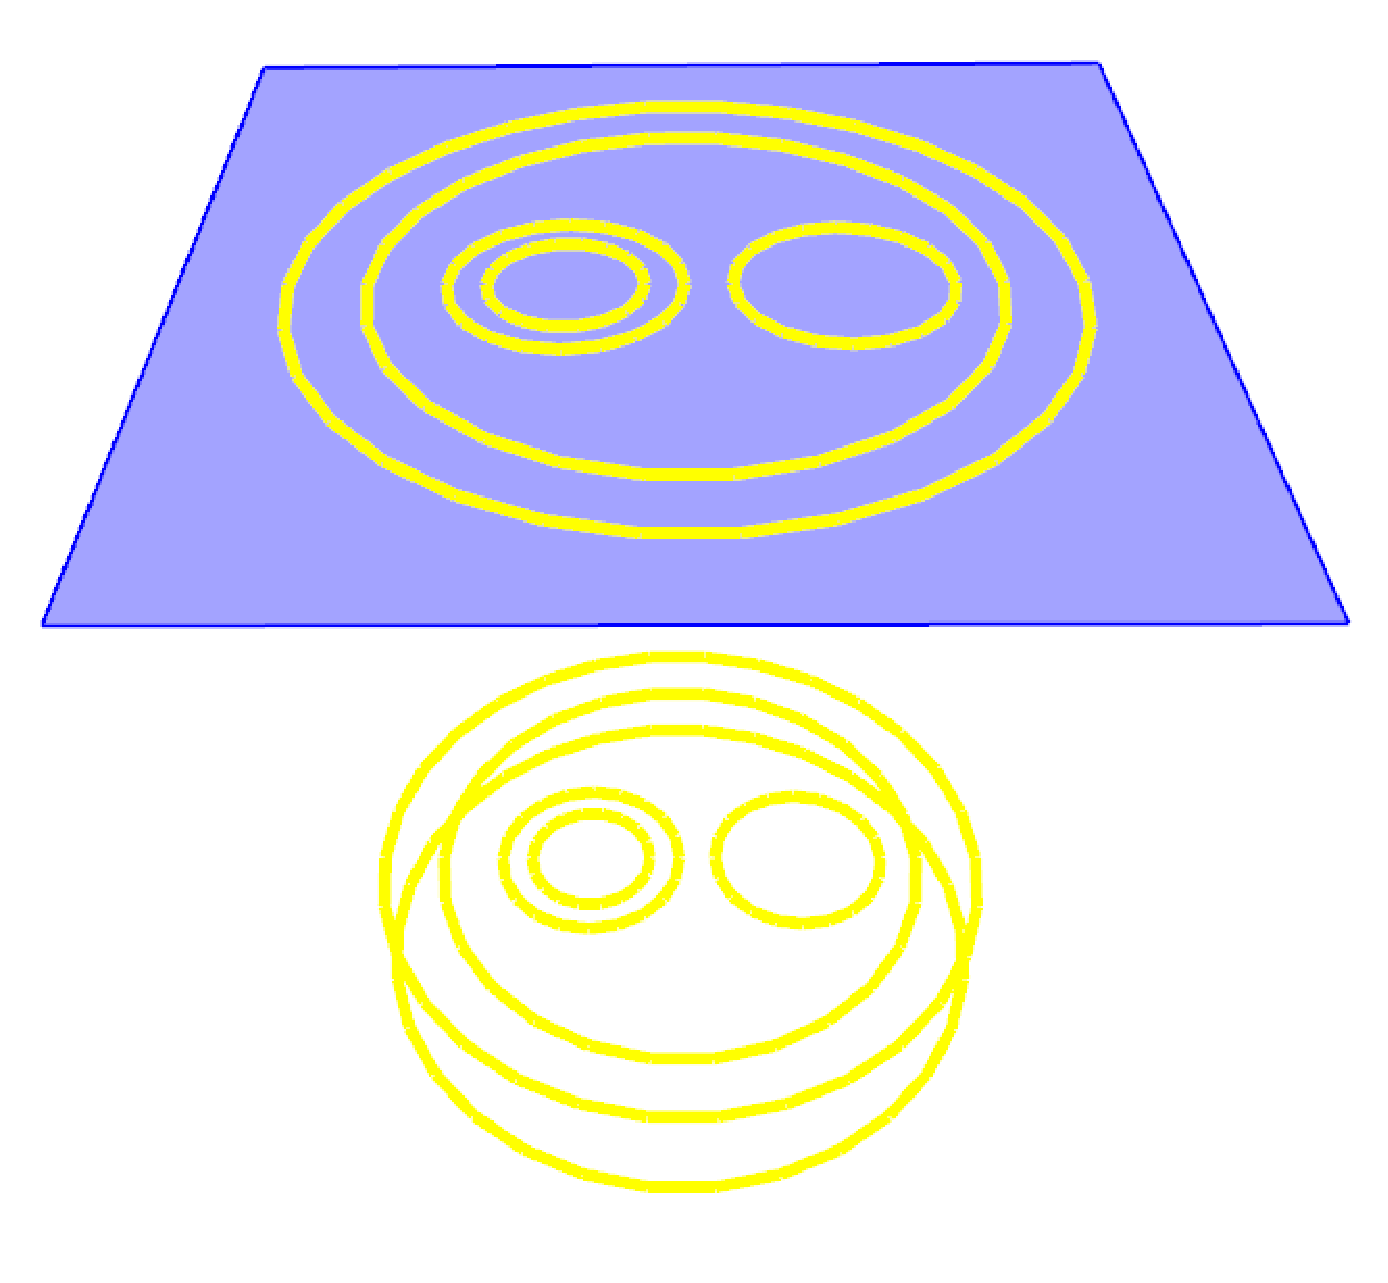
\includegraphics[scale=0.18]{figs/f3.rule2-1.eps}
    \end{minipage}}
  \subfigure[]{
    \centering
    \label{fig:rule2:b}
    \begin{minipage}[b]{0.22\textwidth}
      \centering
      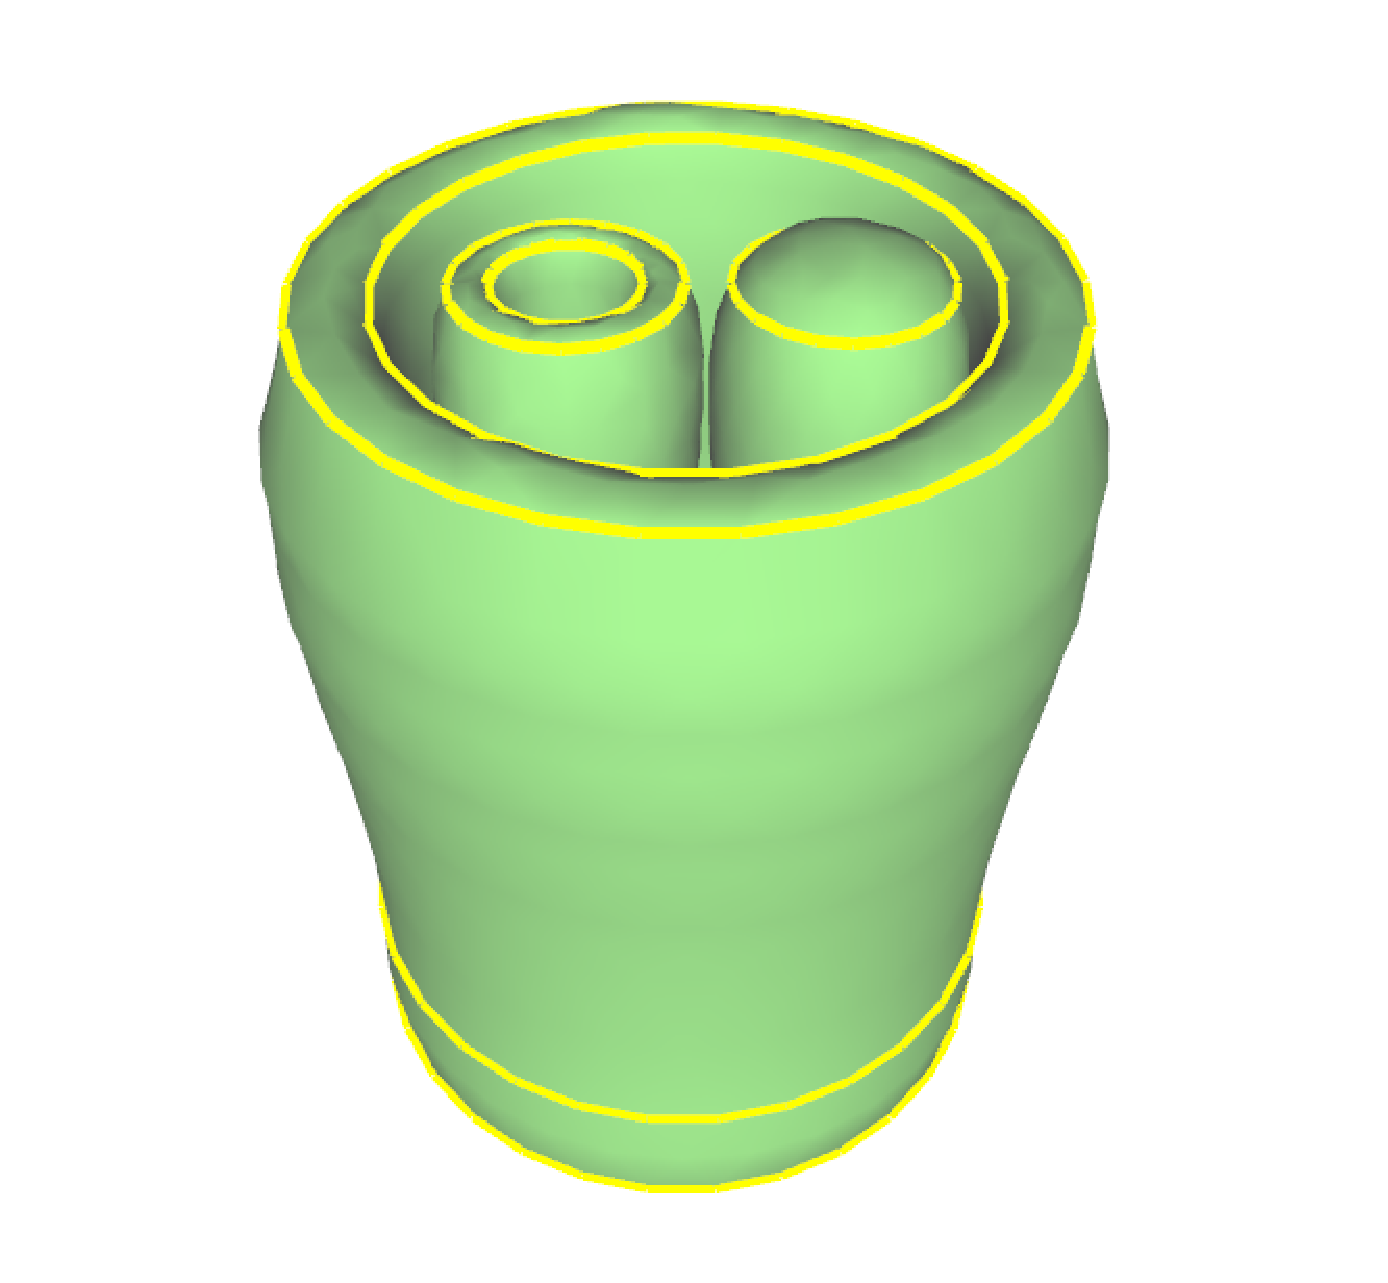
\includegraphics[scale=0.18]{figs/f3.rule2-2.eps}
    \end{minipage}}
  \caption{An example for rule~\ref{rule:2}. (a) The user drawn contours. (b) The generated model.}
  \label{fig:rule2} %% label for entire figure
\end{figure}

Rule~\ref{rule:3} just does not allow self-intersection of one curve or intersection between any two curves on the same plane since it unlikely happens for the cross section contour of an object to have intersection.

Rule~\ref{rule:4} can also be stated in another way that the intersection points between the two curves and the intersection line of the two planes must be be in the same positions. This rule actually conforms to our common understanding of appearance of a 3D object. It is difficult to imagine what the shape of the model will be if the two sets $\{V_{S_1P_2}\}$ and $\{V_{S_2P_1}\}$ are not same. However in practice, it is almost impossible for the users to draw two exactly intersected curves manually. So after the curve $S_1$ is drawn, we highlight the point set $\{V_{S_1P_2}\}$ to help the users carefully draw the curve $S_2$ to make it pass through $\{V_{S_1P_2}\}$. Then we perform a curve deformation procedure, which is explained below, to automatically sew the two curves up before constructing the surface.

For simplicity, let us assume there are two elements in set $\{V_{S_1P_2}\}$, which implies two curves $S_1$ and $S_2$ should intersect at two points. So the goal here is to deform the two curves, making them intersect at two points and meanwhile preserve their original shape as much as possible.

First we calculate the intersection point set $\{V_{S_1P_2}\}$ between $S_1$ and $P_2$, and $\{V_{S_2P_1}\}$ between $S_2$ and $P_1$. Then we find two pairs of different closest points, in each pair the two points are from $\{V_{S_1P_2}\}$ and $\{V_{S_2P_1}\}$ respectively. The midpoints $V_{m1}$ and $V_{m2}$ of these two pairs are treated as the new positions of the handle points. Two handle points on each curve can then be chosen as the points closest to $V_{m1}$ and $V_{m2}$ respectively. Next a range of points near the handles are to be moved with them and we need to compute their new positions. So we could perform the Laplacian deformation algorithm to the two curves to deform them. Since the two curves are both planar, it can be further simplified into a 2D deformation problem which can be precisely solved~\cite{ESA07}.

\begin{figure} [htbp]
  \centering
  \subfigure[]{
    \centering
    \label{fig:curvemerge:a} %% label for first subfigure
    \begin{minipage}[b]{0.25\textwidth}
      \centering
      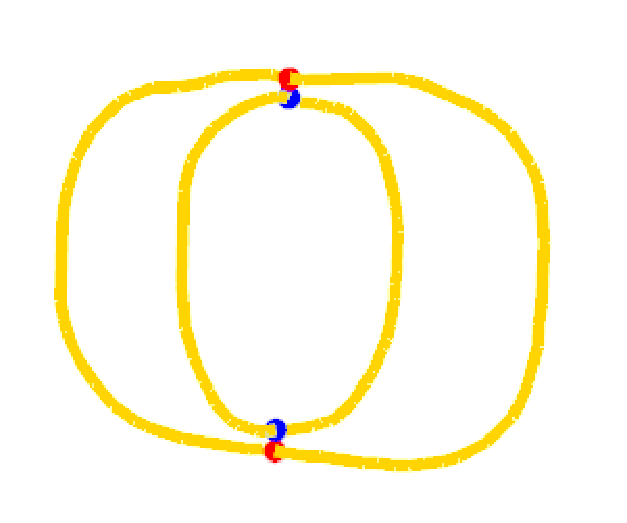
\includegraphics[scale=0.35]{figs/f3.CurveMerge1.eps}
    \end{minipage}}
  \subfigure[]{
    \centering
    \label{fig:curvemerge:b}
    \begin{minipage}[b]{0.25\textwidth}
      \centering
      
\includegraphics[scale=0.35]{figs/f3.CurveMerge2.eps}
    \end{minipage}}
  \subfigure[]{
    \centering
    \label{fig:curvemerge:c}
    \begin{minipage}[b]{0.25\textwidth}
      \centering
      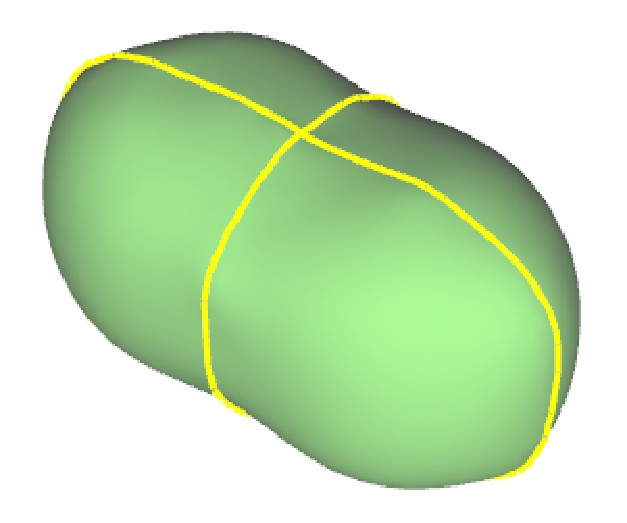
\includegraphics[scale=0.35]{figs/f3.CurveMerge3.eps}
    \end{minipage}}
  \caption{Curve sewing. (a) Two curves lie on two orthogonal planes. The colored points denote the intersection points between a curve and a plane that another curve lies on. (b) Deform the two curves so that they intersect at two points. (c) Generate a mesh that takes the two curves as contours.}
  \label{fig:curvemerge} %% label for entire figure
\end{figure}

It could be seen from Figure~\ref{fig:curvemerge} that during the deformation process, no extra discontinuity will be caused at the intersection part of each curve and the deformed curves keep their original shapes very well, thus preserving the original characteristics of the user input strokes.

The above mentioned steps are for the simple two-contour case. For multiple contours, we just need to deal with them one by one to make them accord with the rules we defined.

After all these processes, we are finally ready to construct the mesh model, which is completed by employing a procedure proposed in ~\cite{LBDLJ08}.

\subsection{Deformation}\label{ch3:sec:alg:deformation}

Since for sketch-based modeling direct manipulation of the mesh surface is expected, we choose the surface-based algorithm for the deformation in our system.

As mentioned in Chapter~\ref{ch3:sec:ui:deformation}, we provide the users reference planes for drawing the deformed shape of the handle curve. A key problem here is how to generate the base plane which has a suitable position and direction, as the projection plane could be easily calculated after the base plane is confirmed.

Our basic assumption is to let the base plane pass through as many points of the handle curve as possible. For this purpose, we compute the least squares plane that fit the points. Assume the plane equation is

\begin{equation}
\label{eq:planefunc}
	Ax+By+Cz+D=0,\nonumber
\end{equation}
where $A$,$B$,$C$ and $D$ are the unknown parameters to be determined. Then our task is to find the plane that minimizes the following objective function

\begin{equation}
\label{eq:planeobjnoZ0}
	f(A,B,C,D)=\sum\limits_{i \in HC} {(Ax_i+By_i+Cz_i-D)^2},
\end{equation}
subject to the constraint $A^2+B^2+C^2=1$, where $i \in HC$ means $p_i=(x_i,y_i,z_i)$ is a point on the handle curve. This optimization problem can be solved using the method proposed in~\cite{SWMB59}.

The above method just gives a suggestive orientation of the base plane. If the user is not satisfied, he/she can rotate the plane by a proper angle. The axis of the rotation is the line connecting the projection of the first handle point onto the initial computed plane to that of the last point. The calculation of the reference plane for extrusion process is the same as this.

After the reference planes are constructed, the user can sketch the new shape and position of the handle curve. If the user intends to draw a non-planar curve by sketching the shadow of the base plane curve on the projection plane, we use the algorithm proposed in~\cite{CMZHB99} to combine the two planar curves to generate a spatial one.

Once the ROI vertices, the handle curve and its new shape are confirmed, a flexible mesh deformation algorithm which can produce various effects between two the Laplacian~\cite{SCLARS04} and Rigid~\cite{SA07} deformation results is used to complete the deformation. The details of the algorithm will be introduced in Chapter~\ref{ch:flexdeformation}.

\subsection{Local Refinement}\label{ch3:sec:alg:refine}

Note that if large deformation is performed, the deformed triangles of the mesh, especially those near the handle vertices, will in general be stretched severely. This will lower the quality of the mesh. To preserve the mesh quality, we introduce a local refinement algorithm that is described below. This algorithm is carried out after each prominent deformation.

\begin{figure} [htbp]
  \centering
  \subfigure[]{
    \centering
    \label{fig:allocalrefine:a} %% label for first subfigure
    \begin{minipage}[b]{0.2\textwidth}
      \centering
      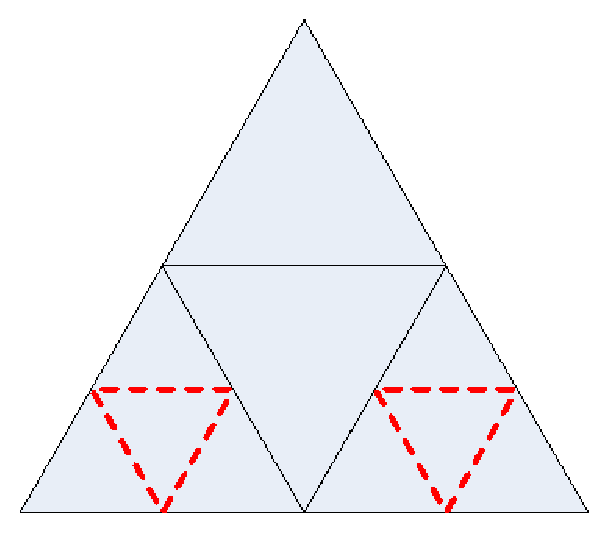
\includegraphics[scale=0.27]{figs/f3.11.a.eps}
    \end{minipage}}
  \subfigure[]{
    \centering
    \label{fig:allocalrefine:b}
    \begin{minipage}[b]{0.2\textwidth}
      \centering
      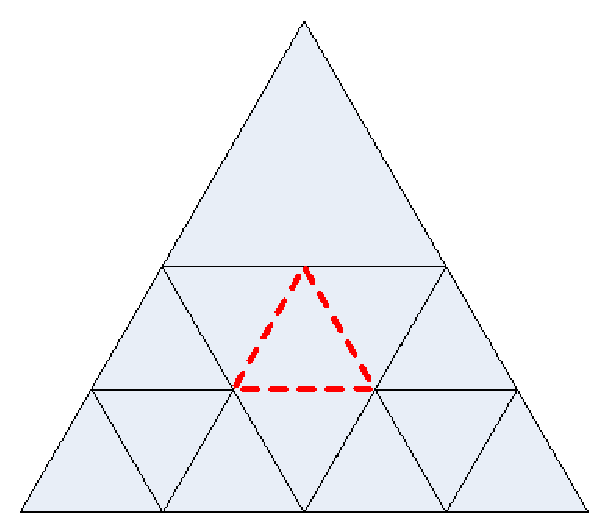
\includegraphics[scale=0.27]{figs/f3.11.b.eps}
    \end{minipage}}
  \subfigure[]{
    \centering
    \label{fig:allocalrefine:c}
    \begin{minipage}[b]{0.2\textwidth}
      \centering
      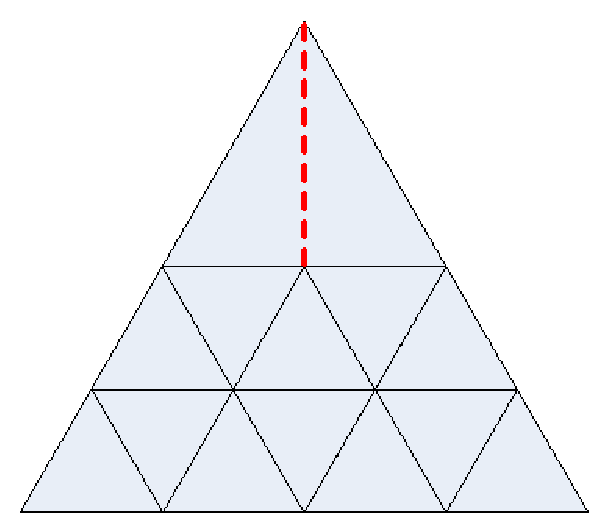
\includegraphics[scale=0.27]{figs/f3.11.c.eps}
    \end{minipage}}
  \subfigure[]{
    \centering
    \label{fig:allocalrefine:d}
    \begin{minipage}[b]{0.2\textwidth}
      \centering
      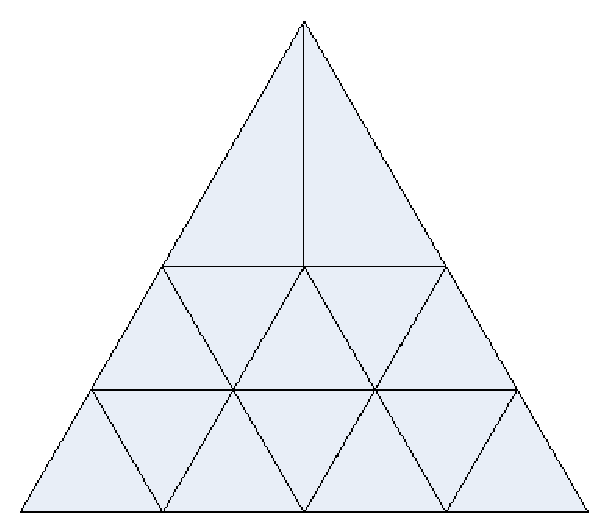
\includegraphics[scale=0.27]{figs/f3.11.d.eps}
    \end{minipage}}
  \caption{Strategy for local refinement. (a) Subdivide the triangle whose centroids move a distance larger than a threshold by connecting the midpoints of the three edges. (b) Iteratively subdivide the triangles that have more than one T-junctions. (c) For the top triangles having only one T-junctions, connect the T-junction to the opposite vertex. (d) The refined mesh.}
  \label{fig:allocalrefine} %% label for entire figure
\end{figure}

The general idea of the local refinement algorithm is to subdivide the original mesh and perform deformation on it, such that the resulting surface will conform to that deformed from the original mesh which is not subdivided and have better quality.

To find out which triangles should be subdivided, we first \textit{virtually} deform the mesh to select the triangles whose centroids move a distance larger than a predefined threshold during deformation. The word \textit{virtually} is used since the change of the surface geometry does not really take effect and the deformation is only used to find the triangles need to be refined at this stage. These triangles are selected since they are supposed to be over-stretched and may probably lower the mesh quality.

So we then subdivide the corresponding triangles on the original mesh by calculating the midpoints of each edge and connecting the new points of the three edges (see Figure~\ref{fig:allocalrefine:a}). Next, for the other neighboring triangles that are not involved in the above refinement, T-junctions will occur at the shared edges. These facets can be further divided into two categories: the triangles with only one and those with two or three T-junction edges. We first choose to deal with the second type by subdividing the triangle in the same way as just mentioned. This process continues recursively until the left triangles all belong to the first type (Figure~\ref{fig:allocalrefine:b}). Finally each of these triangles is remeshed by connecting the T-junction point and the vertex opposite to the edge the T-junction point lies on (Figure~\ref{fig:allocalrefine:c}).

Up to now, all the triangles involved in the local refinement have been determined and the \textit{real} deformation on the refined mesh can be performed to update the geometry of the mesh surface.

\begin{figure} [htbp]
  \subfigure[]{
    \centering
    \label{fig:localrefineEG:a} %% label for first subfigure
    \begin{minipage}[b]{0.25\textwidth}
      \centering
      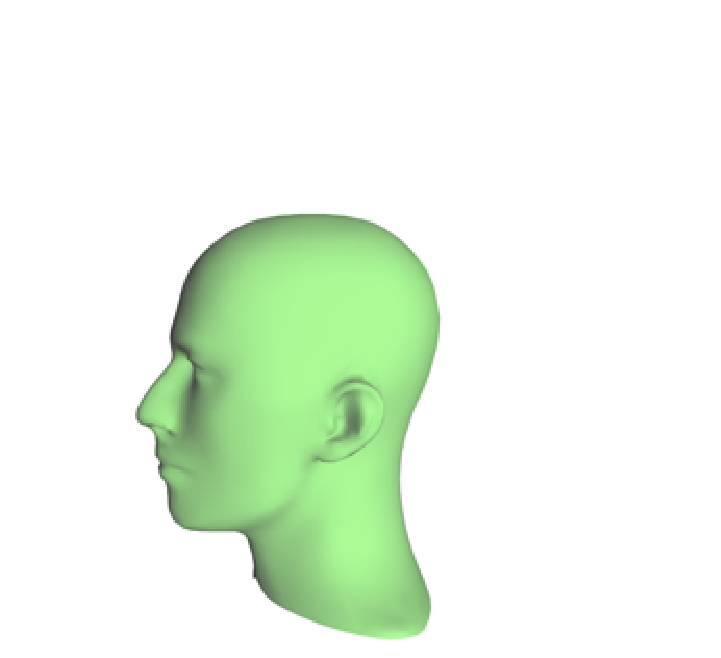
\includegraphics[scale=0.4]{figs/f3.LocalRefineEG1.eps}
    \end{minipage}}
  \subfigure[]{
    \centering
    \label{fig:localrefineEG:b}
    \begin{minipage}[b]{0.35\textwidth}
      \centering
      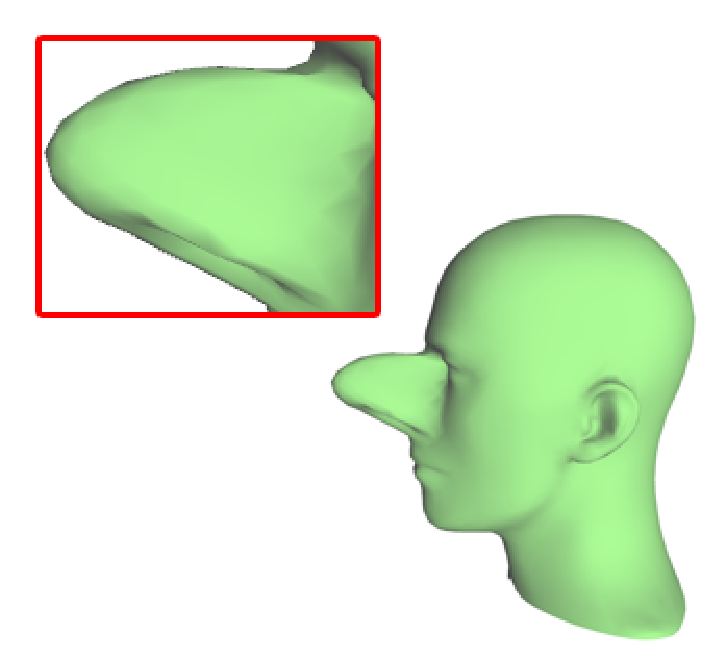
\includegraphics[scale=0.4]{figs/f3.LocalRefineEG2.eps}
    \end{minipage}}
  \subfigure[]{
    \centering
    \label{fig:localrefineEG:c}
    \begin{minipage}[b]{0.35\textwidth}
      \centering
      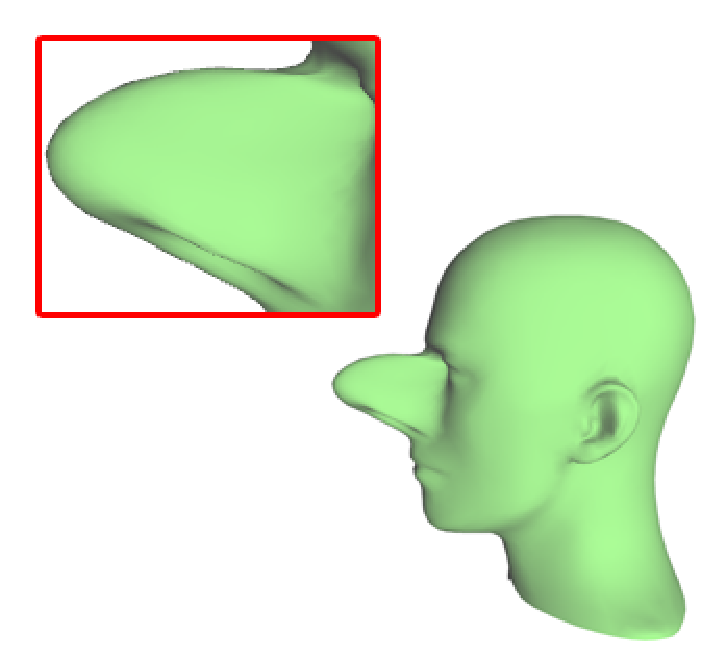
\includegraphics[scale=0.4]{figs/f3.LocalRefineEG3.eps}
    \end{minipage}}
  \caption{An example of local refinement after large deformation. (a) The initial model. (b) Result after large deformation without local refinement. (c) Result after large deformation with local refinement.}
  \label{fig:localrefineEG} %% label for entire figure
\end{figure}

This simple local refinement algorithm works well in our system for improving the quality of the mesh after large deformations, as can be seen in Figure~\ref{fig:localrefineEG}. It should also be pointed out that this remeshing process fits for a local area, whereas most of the other popular remeshing algorithms are applied to the whole mesh.

%\subsection{Others}\label{ch3:sec:alg:others}
%
%It has been mentioned in Section~\ref{ch3:sec:ui:others} that in the extrusion function we provide the users with a reference plane for drawing the silhouette curve on. For the calculation of this reference plane, we first compute the least-square plane for the closed curve projected from the 2D user drawings onto the mesh, through~\ref{eq:planeobjnoZ0}. Then the reference plane is chosen as a plane orthogonal to the calculated one. To confirm the specific orientation, we calculated projection of the first point and the centroid of the closed curve onto the best-fitting plane and let the reference plane pass through these two projection points. This way, an initial reference plane is uniquely specified. As has been introduced, this reference plane could be further rotated along two axes to a satisfactory angle.
%
%After the silhouette curve has been drawn, we use the method of Teddy~\cite{IMT99} to extrude the circled part of the mesh out along the silhouette curve. After this extrusion, we implement the Laplacian smoothing algorithm to the joint region of the mesh and the extruded part to make it visually fair enough.
%
%The algorithm for the cutting function is the same as in Teddy. And the supporting algorithm we use for the smoothing function is the famous $\lambda | \mu$ mesh smoothing algorithm proposed in~\cite{TG95}. This is because it prevents the shrinkage of the surface and is quick enough for interactive applications.

\section{Results and Discussions}\label{ch3:sec:result}

\begin{figure} [htbp]
\renewcommand{\thesubfigure}{}
%\renewcommand{\@thesubfigure}{}
  \centering
  \subfigure[]{
    \centering
    \label{fig:results:a} %% label for first subfigure
    \begin{minipage}[b]{0.38\textwidth}
      \centering
      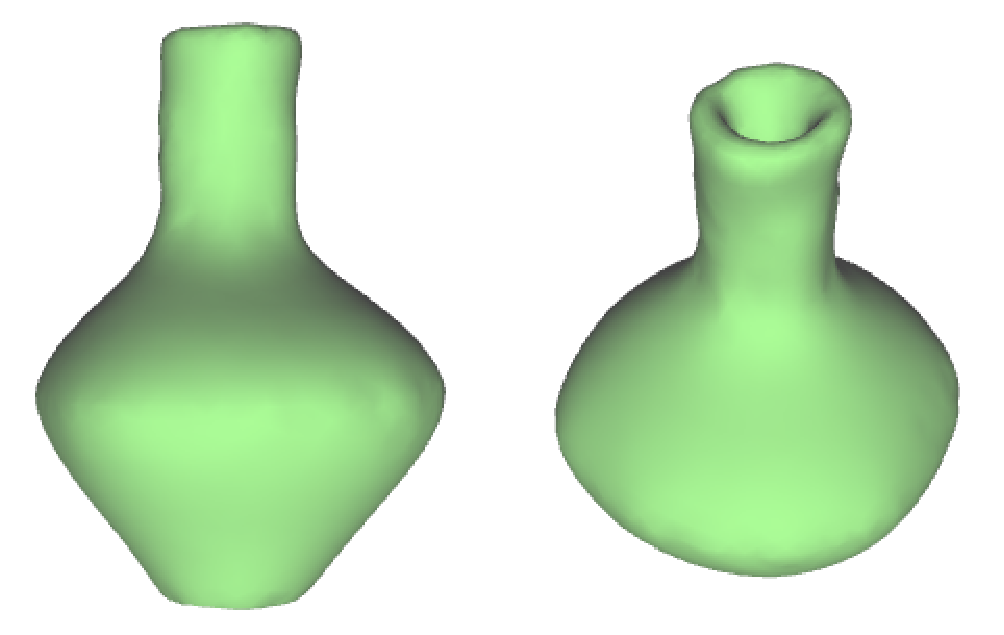
\includegraphics[scale=0.33]{figs/f3.bottle.eps}
    \end{minipage}}
  \subfigure[]{
    \centering
    \label{fig:results:b}
    \begin{minipage}[b]{0.5\textwidth}
      \centering
      \includegraphics[scale=0.33]{figs/f3.car.eps}
    \end{minipage}}
    \\
  \subfigure[]{
    \centering
    \label{fig:results:c}
    \begin{minipage}[b]{0.48\textwidth}
      \centering
      \includegraphics[scale=0.22]{figs/f3.mushroom.eps}
    \end{minipage}}
  \subfigure[]{
    \label{fig:results:d}
    \begin{minipage}[b]{0.48\textwidth}
      \centering
      \includegraphics[scale=0.22]{figs/f3.pig.eps}
    \end{minipage}}
    \\
  \subfigure[]{
    \label{fig:results:e}
    \begin{minipage}[b]{0.5\textwidth}
      \centering
      \includegraphics[scale=0.28]{figs/f3.plane.eps}
    \end{minipage}}
  \subfigure[]{
    \label{fig:results:f}
    \begin{minipage}[b]{0.38\textwidth}
      \centering
      \includegraphics[scale=0.36]{figs/f3.fish.eps}
    \end{minipage}}
  \caption{Some models created by our system in two views.}
  \label{fig:results} %% label for entire figure
\end{figure}

We have implemented our sketch-based modeling system. Our current implementation was written in C++ on the Windows platform. We tested out system on an Intel Pentium 4 3.6GHz machine with 1G RAM. Our experiments show that each operation of our system runs in interactive rates. This indeed meets the users' requirement on a sketch-based modeling system.

Several 3D freeform models created with our system are shown in Figure~\ref{fig:results}. Since the sketching tool in our system provides the freedom of sketching in 3D space, which is different from other systems that only enable the drawing on the 2D screen, the modeling becomes much intuitive and flexible.

With our system, many 3D objects with complex topology could be created at the creation stage. With help of reference planes, the sculpting process at the subsequent editing stage can also be speeded up to a large extent. This is due to precise awareness of the position and orientation of 3D sketches.

It is observed in our experiment that even if multiple cross section curves are defined initially, the constructed mesh is not quite dense and the number of vertices is about a few hundreds. Even after complex editing operations, this number is still no more than a few thousands. This enables us to consider more about the modeling effect and quality of the mesh other than the running time. Such an example can be found at our local refinement algorithm after deformation. Since the remeshing will change the connectivity of the mesh, the re-calculation and re-factorization of the $n \times n$ matrix when solving the deformation problem is often inevitable ($n$ refers to the number of vertices involved). This task can still be performed in real-time thanks to the small number of vertices of the model.


\section{Summary}\label{ch3:sec:sum}

We have described a novel sketching interface for creating and editing 3D models. The main contributions are:

\begin{itemize}
	\item We propose the strategy of using auxiliary planes as references for creation, deformation and other editing operations in sketching interface. Reference planes help make the sketch-based modeling process intuitive and easy to use.
	\item We propose some rules for regularizing and interpreting the user input sketches. These rules consider both the semantic meaning of the sketched strokes and human psychology.
	\item We introduce a local mesh refinement procedure to improve the quality of the deformed mesh.
\end{itemize}

In future, we will explore the use of more types of geometry objects as references to assist sketch-based interface and modeling. In addition, more advanced local remeshing algorithms are needed to improve the quality of meshes after large deformations.